%%%%%%%%%%%%%%%%%%%%%%%%%%%%%%%%%%%%%%%%%%%%%%%%%%%%%%%%%%%%%%%%%%%%%%%%%
%%   CHAPTER: THE 0E0P METACELL
%%%%%%%%%%%%%%%%%%%%%%%%%%%%%%%%%%%%%%%%%%%%%%%%%%%%%%%%%%%%%%%%%%%%%%%%%

\renewcommand{\chapterfolder}{0e0p/}
\chapterimage{cover/0e0p}
\chapter{The 0E0P Metacell}\label{chp:0e0p}\index{0E0P metacell}


\vspace*{-0.4in}
\epigraph{If you couldn't predict what [Life] did then probably that's because it's capable of doing anything.}{John H. Conway}
\vspace*{0.15in}


\noindent In the previous chapter, we introduced universal construction and presented several adjustable spaceships based on it. In this chapter, we explore a more complex application of universal construction: a self-reproducing pattern that interacts with nearby copies of itself so as to emulate Conway's Game of Life, or a different cellular automaton, on a much larger and slower scale.

Specifically, we construct a pattern called the \textbf{0E0P metacell},\footnote{Constructed by Adam P.~Goucher from 2014 to November 2018. The acronym ``0E0P'' stands for ``(State) 0 Encoded by 0 Population'', in reference to the fact that its ``off'' state is just a metacell-sized region of empty space---its most remarkable property, which is not shared by any metacell that came before it (see Section~\ref{sec:0e0p_history}).} which has the property that if we arrange copies of it on the Life plane then, at a zoomed-out macroscopic scale, it evolves in the same way that the corresponding arrangement of cells would evolve. For example, if we place five copies of this metacell in the Life plane in the formation of a glider, as illustrated in Figure~\ref{fig:0e0p_glider}, then we indeed get a spaceship that travels like a glider (but much more slowly).

\begin{figure}[!htb]
	\centering
	\embedlink{0e0p_glider}{\vcenteredhbox{\patternimg{0.129}{0e0p_glider_0}} \vcenteredhbox{\color{black}{$\xrightarrow{\text{\clock{4}{45} $2^{36}$}}$}} \vcenteredhbox{\patternimg{0.129}{0e0p_glider_236}}}
	\caption{A \textbf{metaglider}\index{metaglider} made up of five copies of the 0E0P metacell, each of which is $2^{18} \times 2^{18}$ and logically makes up one ``cell''. It travels in much the same way as a glider, but $2^{36}$ times as slowly.}\label{fig:0e0p_glider}
\end{figure}

A meta-fied pattern like this is roughly $2^{18} = 262{\thousep}144$ times as large as the original pattern that it is based on, and it runs $2^{36} = 68{\thousep}719{\thousep}476{\thousep}736$ times as slowly. Indeed, the 0E0P metacell is so much larger and slower than any other pattern that we have seen in this book that evolving the metaglider from Figure~\ref{fig:0e0p_glider} through four \textbf{metagenerations}\index{metageneration} (i.e., $4 \times 2^{36}$ generations), to see that it really is a spaceship, would take a couple of years on a modern desktop computer via standard Life simulation algorithms.\footnote{The fastest ``standard'' Life simulation algorithm is \textbf{HashLife} \cite{Gos84}, which is fast enough to run any of the patterns that we saw earlier in this book---even huge ones like the $\pi$ calculator and the Gemini spaceship. To run patterns that use huge streams of gliders (like the 0E0P metacell) more efficiently, Adam P.~Goucher developed a new \textbf{StreamLife} algorithm, but even it would require several months to evolve a metaglider through four metagenerations.}\index{HashLife}\index{StreamLife}

While emulating Life within Life perhaps does not seem as remarkable a feat as some of the other things we have achieved over the past three chapters, what really makes the 0E0P metacell shine is that it can actually emulate a huge variety of 2D cellular automata besides Life as well. As a result, any pattern from one of those other cellular automata can be straightforwardly ``imported'' into Life simply by meta-fying it, thus giving us exotic new types of patterns that were previously not known how to construct.

To illustrate this phenomenon, consider the cellular automaton that has all the same rules as Life, plus the additional rule that a dead cell comes to life if it has exactly $6$ live neighbors (i.e., the Life-like cellular automaton with rulestring\index{rulestring} \texttt{B36/S23}). This cellular automaton is called \textbf{HighLife},\index{HighLife} and it is interesting for the fact that it has a simple \textbf{replicator}:\index{replicator (pattern)} a pattern that produces arbitrarily many copies of itself, as illustrated in Figure~\ref{fig:highlife_replicator}.

\begin{figure}[!htb]
	\centering
	\embedlink{highlife_replicator}{\vcenteredhbox{\patternimg{0.122}{highlife_replicator_0}} \vcenteredhbox{\genarrow{12}} \vcenteredhbox{\patternimg{0.122}{highlife_replicator_12}} \vcenteredhbox{\genarrow{12}} \vcenteredhbox{\patternimg{0.122}{highlife_replicator_24}} \vcenteredhbox{\genarrow{12}} \vcenteredhbox{\patternimg{0.122}{highlife_replicator_36}}}
	\caption{A \textbf{replicator} in the HighLife (\texttt{B36/S23}) Life-like cellular automaton that duplicates itself every $12$~generations. Found by Nathan Thompson in February 1994.}\label{fig:highlife_replicator}
\end{figure}

After this replicator copies itself the first time, each of its copies attempt to do the same. However, since these copies are right next to each other, two of \emph{their} copies attempt to occupy the same space, and instead annihilate each other (while their other copies are successfully created farther away). This behavior repeats forever: every $12$~generations, if there is space for a copy of this replicator then it is made, but two copies being made at the same spot at the same time mutually annihilate. The result is that after $n$ replication cycles (i.e., at generation $12n$), the number of replicators is exactly $2^{B(n)}$, where $B(n)$ is the \textbf{binary weight}\index{binary weight} of $n$: the number of ``1'' bits in its binary representation.

Since we're using HighLife's rules that require birth when a dead cell has $6$ live neighbors, this is not a valid replicator in Life: when run, it merely degenerates into a configuration of eight blinkers. However, we can ``import'' its behavior into regular Life by programming the 0E0P metacell to emulate HighLife and then arranging $12$ copies of that metacell in the same formation as the $12$~cells that make up the replicator from Figure~\ref{fig:highlife_replicator}. This meta-fied replicator is displayed in Figure~\ref{fig:meta_replicator}.\footnote{Slsparse (see \httpsurl{conwaylife.com/wiki/Slsparse}) comes with a Python script called \texttt{isotropic\_metafier.py} that can metafy patterns like this automatically.} While it is not the first replicator to be constructed in Life (that honor goes to the linear propagator\index{linear propagator} that we mentioned in Section~\ref{sec:universal_construction_history}), this is just the tip of the monumental iceberg of what can be done with the 0E0P metacell.

\begin{figure}[!htb]
	\centering
	\embedlink{metareplicator}{\vcenteredhbox{\patternimg{0.135}{metareplicator_0}} \vcenteredhbox{\color{black}{$\xrightarrow{\text{\clock{4}{55} $12 \times 2^{36}$}}$}} \vcenteredhbox{\patternimg{0.135}{metareplicator_12}}}
	\caption{A replicator in Conway's Game of Life that is made up of twelve 0E0P metacells, each emulating the HighLife rule (\texttt{B36/S23}) from Figure~\ref{fig:highlife_replicator}.}\label{fig:meta_replicator}
\end{figure}

In this chapter, we first explore a few other cellular automata that have exotic patterns that can be implemented in this way in Life via the 0E0P metacell, and then we describe the inner workings of the 0E0P metacell itself.


%%%%%%%%%%%%%%%%%%%%%%%%
\section{Other 2D Cellular Automata}\label{sec:other_ca_rules}\index{cellular automaton}
%%%%%%%%%%%%%%%%%%%%%%%%

While cellular automata (CA)\index{CA|see {cellular automaton}} can act on grids of any dimension and of a variety of different shapes, all of the ones that we consider (and all of the ones that can be emulated by the 0E0P metacell) act on a 2-dimensional square grid. Furthermore, in this section we only consider cellular automata that use two states, which we still refer to as ``alive'' and ``dead'', and the Moore neighborhood of Figure~\ref{fig:neighborhood}, though we will see in Section~\ref{sec:0e0p_rule_emulation} that the 0E0P metacell can emulate some cellular automata without these two restrictions.


%%%%%%%%%%%%%%%%%%%%%%%%
\subsection{Life-Like (i.e., Outer-Totalistic) Cellular Automata}\label{sec:lifelike_rules}\index{Life-like}\index{outer-totalistic}\index{totalistic}
%%%%%%%%%%%%%%%%%%%%%%%%

A $2$-state cellular automaton is called \textbf{outer-totalistic} if the birth and death rules depend only on the state of the current cell, as well the number of live neighbors that it has.\footnote{In contrast with \textbf{totalistic} cellular automata, in which the birth and death rules depend only on the number of live neighbors including the cell itself.} That is, they are exactly the cellular automata that can be described by the \texttt{Bx/Sy} rulestring\index{rulestring} notation that was introduced earlier. An outer-totalistic cellular automaton is said to be \textbf{Life-like} if it furthermore satisfies all of the properties that we assumed at the start of this section (i.e., it acts on a 2-dimensional square grid and neighbors are counted according to the Moore neighborhood).

Some Life-like cellular automata have simple patterns that behave unlike any simple patterns that are known in Life itself, as evidenced by the replicator that we saw in Figure~\ref{fig:highlife_replicator}. While that pattern replicates along a single line, there are also Life-like rules that give rise to simple replicators that replicate in multiple directions and fill the whole plane. In fact, in the appropriately-named \textbf{replicator}\index{replicator (rule)} rule (\texttt{B1357/S1357}), \emph{every} pattern is a replicator that repeatedly produces copies of itself in all $8$ orthogonal and diagonal directions---see Figure~\ref{fig:replicator_smile} and Exercise~\ref{exer:replicator_rule_really_replicates}.

\begin{figure}[!htb]
	\centering
	\embedlink{replicator_smile}{\vcenteredhbox{\patternimg{0.19495412844}{replicator_smile_0}} \vcenteredhbox{\genarrow{8}} \vcenteredhbox{\patternimg{0.11486486484}{replicator_smile_8}} \vcenteredhbox{\genarrow{8}} \vcenteredhbox{\patternimg{0.06789137379}{replicator_smile_16}} \vcenteredhbox{\genarrow{8}} \vcenteredhbox{\patternimg{0.0927947598}{replicator_smile_24}}}
	\caption{In the \textbf{replicator} rule (\texttt{B1357/S1357}), every pattern is a replicator that creates copies of itself in the $8$ standard directions.}\label{fig:replicator_smile}
\end{figure}

While the patterns of Figures~\ref{fig:highlife_replicator} and~\ref{fig:replicator_smile} replicate in a sawtooth-like\index{sawtooth} fashion---whenever two copies would be created in the same place, they cleanly destroy each other instead, so their populations repeatedly reach new heights and then jump back down below some fixed value---replicators need not behave in this way. For example, consider the rule \texttt{B12345678/S012345678} in which a  cell is born if it ever has at least one live neighbor, and then lives forever. In this rule, a single cell acts as a replicator that repeatedly births all cells in its Moore neighborhood, as illustrated in Figure~\ref{fig:all_births_replicator}.

\begin{figure}[!htb]
	\centering
	\embedlink{replicator_all_births}{\vcenteredhbox{\patternimg{0.11}{replicator_all_births_0}} \vcenteredhbox{\genarrow{1}} \vcenteredhbox{\patternimg{0.11}{replicator_all_births_1}} \vcenteredhbox{\genarrow{1}} \vcenteredhbox{\patternimg{0.11}{replicator_all_births_2}} \vcenteredhbox{\genarrow{1}} \vcenteredhbox{\patternimg{0.11}{replicator_all_births_3}}}
	\caption{A single cell acts as a space-filling replicator in the rule \texttt{B12345678/S012345678}.}\label{fig:all_births_replicator}
\end{figure}

In fact, elementary replicators of various shapes and speeds are known in a few dozen different Life-like cellular automata,\footnote{See \httpsurl{www.ics.uci.edu/~eppstein/ca/replicators/index.html} for a partial list.} giving us a wide variety of patterns of this type in Life now, thanks to the 0E0P metacell. Somewhat less common are patterns that grow in other ways, like the spiral-growth pattern\index{spiral growth} for the rule \texttt{B34568/S15678} that is displayed in Figure~\ref{fig:spiral_growth_elementary} (compare with the spiral growth pattern that we constructed in Life back in Figure~\ref{fig:spiral_growth}).

\begin{figure}[!htb]
	\centering
	\embedlink{spiral_growth_elementary}{\vcenteredhbox{\patternimg{0.123}{spiral_growth_elementary_0}} \vcenteredhbox{\genarrow{12}} \vcenteredhbox{\patternimg{0.123}{spiral_growth_elementary_1}} \vcenteredhbox{\genarrow{12}} \vcenteredhbox{\patternimg{0.123}{spiral_growth_elementary_13}} \vcenteredhbox{\genarrow{12}} \vcenteredhbox{\patternimg{0.123}{spiral_growth_elementary_25}} \vcenteredhbox{\genarrow{12}} \vcenteredhbox{\patternimg{0.123}{spiral_growth_elementary_37}}}
	\caption{A pattern that exhibits spiral growth in the \texttt{B34568/S15678} rule. Found by Dean Hickerson in June 2006.}\label{fig:spiral_growth_elementary}
\end{figure}


%%%%%%%%%%%%%%%%%%%%%%%%
\subsection{Isotropic (but Non-Outer-Totalistic) Cellular Automata}\label{sec:isotropic_rules}\index{isotropic}\index{non-isotropic}
%%%%%%%%%%%%%%%%%%%%%%%%

A cellular automaton is called \textbf{isotropic} if the cell transition rules are invariant under rotations and reflections, and it is called \textbf{non-isotropic} otherwise. That is, an isotropic cellular automaton may take into account the \emph{relative} positions of neighboring cells, but not their \emph{absolute} positions. Every outer-totalistic cellular automaton is isotropic, but the converse is not true, as shown in Figure~\ref{fig:isotropic_neighborhoods}.

\begin{figure}[!htb]
	\centering
	\patternimg{0.15}{isotropic_neighborhoods}
	\caption{In an outer-totalistic cellular automaton, the central cells (displayed in \bgbox{orangeback}{orange}) in the leftmost four configurations must all evolve in the same way, since they have the same number of live neighbors ($2$). In an isotropic cellular automaton, the central cells must evolve in the same way in only the \emph{three} leftmost configurations, since their arrangements of neighbors are rotations and/or reflections of each other. In a non-isotropic cellular automaton, the central cells can evolve in different ways in all five configurations.}\label{fig:isotropic_neighborhoods}
\end{figure}

Because of the extra flexibility afforded by isotropic cellular automata (there are a whopping $2^{102}$ isotropic $2$-state CA on a 2D square grid, versus ``just'' $2^{18}$ outer-totalistic ones), they often contain elementary patterns that appear completely alien when compared to those from Life. For example, consider the CA that has the same rules as Life, but with four isotropic modifications: two to its birth conditions and two to its survival conditions, as illustrated in Figure~\ref{fig:iso_rule_modifications}. This CA's rulestring is \texttt{B3-j6i/S23-c4i}, where the substrings ``\texttt{-j}'', ``\texttt{6i}'', ``\texttt{-c}'', and ``\texttt{4i}'' correspond to these four new rules (in the same order as they are displayed in Figure~\ref{fig:iso_rule_modifications}). The details of how to construct rulestrings for arbitrary isotropic cellular automata are somewhat involved, so we leave them to Appendix~\ref{sec:isotropic_rulestrings}.

\begin{figure}[!htb]
	\centering
	\patternimg{0.15}{iso_rule_modifications}
	\caption{The four differences (up to rotation and reflection) between Life (\texttt{B3/S23}) and the isotropic cellular automaton \texttt{B3-j6i/S23-c4i}. The central cell in the first (i.e., leftmost) configuration is \emph{not} born (whereas it would be in Life), the central cell is born in the next configuration, the central cell dies in the third, and the central cell survives in the fourth.}\label{fig:iso_rule_modifications}
\end{figure}

Our interest in this cellular automaton comes from the pattern displayed in Figure~\ref{fig:reflectorless_rotating_oscillator}, which is an example of a \textbf{reflectorless rotating oscillator}\index{reflectorless rotating oscillator} (or \textbf{RRO}\index{RRO|see {reflectorless rotating oscillator}} for short): an oscillator with the property that one of its phases is a rotation of another one, and two non-interacting copies of the oscillator can combine so as to produce an oscillator with period half as large.\footnote{This final ``two copies...'' requirement enforces the ``reflectorless'' part of the name: a single glider in a square Snark loop is an oscillator whose phases are rotations of other phases, but two copies of this loop only produce an oscillator with half the period if we overlap the Snarks (thus violating the ``non-interacting'' part of the definition of an RRO).} Informally, RROs travel around in a loop like a spaceship that periodically turns a corner (they are even sometimes called \textbf{looping spaceships}).\index{looping spaceship|see {reflectorless rotating oscillator}} This is very unlike anything that we have seen in Life---all oscillators that we have seen either stay mostly stationary (like all of the oscillators in the first 8 or 9 pages of Chapter~\ref{chp:oscillators}), or move around a path with the help of other stationary pieces (like glider loops, Herschel tracks, and the pi-heptomino hassler from Figure~\ref{fig:p37_pi_hassler}).

\begin{figure}[!htb]
	\centering
	\begin{subfigure}{.32\textwidth}
		\centering
		\patternimglink{0.079}{reflectorless_rotating_oscillator}
		\caption{One copy, period $200$.}
		\label{fig:reflectorless_rotating_oscillator1}
	\end{subfigure} \hfill % 
	\begin{subfigure}{.32\textwidth}
		\centering
		\patternlink{reflectorless_rotating_oscillator}{\patternimg{0.079}{reflectorless_rotating_oscillator2}}
		\caption{Two copies, period $100$.}
		\label{fig:reflectorless_rotating_oscillator2}
	\end{subfigure} \hfill % 
	\begin{subfigure}{.32\textwidth}
		\centering
		\patternlink{reflectorless_rotating_oscillator}{\patternimg{0.079}{reflectorless_rotating_oscillator4}}
		\caption{Four copies, period $50$.}
		\label{fig:reflectorless_rotating_oscillator4}
	\end{subfigure}
	\caption{A \textbf{reflectorless rotating oscillator} in the isotropic cellular automaton \texttt{B3-j6i/S23-c4i}. Either one, two, or four copies of the oscillator can be placed along the same path, producing oscillators with periods 200, 100, and 50. Found by ConwayLife.com forums user ``Hdjensofjfnen'' in January 2020.}\label{fig:reflectorless_rotating_oscillator}
\end{figure}

Another exotic type of pattern that appears in isotropic cellular automata, but for which no elementary example is known in their Life-like brethren, is a \textbf{spaceship made of spaceships}\index{spaceship made of spaceships} (or \textbf{SMOS}\index{SMOS|see {spaceship made of spaceships}} for short): a spaceship that works by colliding two or more other spaceships with each other.\footnote{The Demonoids\index{Demonoid} that we constructed in the previous chapter are \emph{mostly} made up of gliders. However, they are not spaceships made of spaceships since there is no phase in which they consist \emph{entirely} of gliders.} One of the simplest such patterns occurs in the (admittedly very \emph{not} simple) cellular automaton
\begin{center}
	\texttt{B3acijn4jktwyz5ijr6-en7c/S2aen3-aceq4acijqty5cikr6ak7c}.
\end{center}
Under this rule, a glider functions as a $c/4$ diagonal spaceship in the exact same way as in Life, but if two gliders collide together just right then they push each other in such as way as to produce a $4c/17$ orthogonal spaceship (see Figure~\ref{fig:smos}). Even more remarkably, if two of these $4c/17$ spaceships collide together just right then they produce a $c/44$ diagonal spaceship---a \textbf{spaceship made of spaceships made of spaceships}\index{spaceship made of spaceships made of spaceships} (\textbf{SMOSMOS}).\index{SMOSMOS|see {spaceship made of spaceships made of spaceships}}

\begin{figure}[!htb]
	\centering
	\begin{subfigure}{.32\textwidth}
		\centering
		\embedlink{smosmos}{\patternimg{0.1226519337}{smos_glider}}
		\caption{A ($c/4$ diagonal) glider.}
		\label{fig:smos_glider}
	\end{subfigure} \hfill % 
	\begin{subfigure}{.32\textwidth}
		\centering
		\patternlink{smosmos}{\patternimg{0.1226519337}{smos}}
		\caption{A $4c/17$ orthogonal SMOS.}
		\label{fig:smos_smos}
	\end{subfigure} \hfill % 
	\begin{subfigure}{.32\textwidth}
		\centering
		\patternlink{smosmos}{\patternimg{0.12}{smosmos}}
		\caption{A $c/44$ diagonal SMOSMOS.}
		\label{fig:smos_smosmos}
	\end{subfigure}
	\caption{In the rule \texttt{B3acijn4jktwyz5ijr6-en7c/S2aen3-aceq4acijqty5cikr6ak7c}, (a) a glider functions as a $c/4$ diagonal spaceship in the usual way. However, when it collides with itself it turns into (b) a $4c/17$ orthogonal spaceship (found by ConwayLife.com forums user ``Saka'' in August 2017), and when \emph{that} spaceship collides with itself it turns into (c) a $c/44$ diagonal spaceship (found by ConwayLife.com forums user ``FWKnightship'' in August 2019).}\label{fig:smos}
\end{figure}


%%%%%%%%%%%%%%%%%%%%%%%%
\subsection{Non-Isotropic Cellular Automata}\label{sec:non_isotropic_rules}\index{non-isotropic}
%%%%%%%%%%%%%%%%%%%%%%%%

If we go one step further and consider non-isotropic cellular automata, we can make even just a single cell behave in an extraordinary variety of ways. For example, we can define a rule with the property that cells never survive, and they are only born if they have a single live cell directly to their left.\footnote{This cellular automaton is described by the rulestring\protect\\\texttt{MAPAAAAAIAAAAAAAAAAAAAAAAAAAAAAAAAAAAAAAAAAAAAAAAAAAAAAAAAAAAAAAAAAAAAAAAAAAAAAAAAAAAAAAA}.\protect\\ For an explanation of rulestrings of non-isotropic cellular automata, see Appendix~\ref{sec:non_isotropic_rulestrings}.} In this rule, a single cell is a spaceship that travels orthogonally at lightspeed (see Figure~\ref{fig:single_cell_orth}).

We can also consider the slightly more exotic cellular automaton in which cells are only born if they have no neighbors or a single neighbor to their southeast, and they only survive if they have neighbors everywhere \emph{except} for to their north and northwest.\footnote{This cellular automaton is described by the rulestring\protect\\\texttt{MAPwAAAAAAAAAAAAAAAAAAAAQAAAAAAAAAAAAAAAAAAAAAAAAAAAAAAAAAAAAAAAAAAAAAAAAAAAAAAAAAAAAAAAA}.} In this rule, a single cell acts as a $(1,2)c/2$ knightship,\index{knightship} as illustrated in Figure~\ref{fig:single_cell_knightship}. It is similarly possible to construct rules in which a single cell is a spaceship that travels at many other speeds and slopes---see Exercise~\ref{exer:0e0p_single_cell_spaceships}.

\begin{figure}[!htb]
	\centering
	\begin{subfigure}{.32\textwidth}
		\centering
		\patternimglink{0.15}{single_cell_orth}
		\caption{A single-cell lightspeed orthogonal spaceship.}
		\label{fig:single_cell_orth}
		\begin{minipage}{.1cm}
			\vfill
		\end{minipage}
	\end{subfigure} \hfill % 
	\begin{subfigure}{.65\textwidth}
		\centering
		\embedlink{single_cell_knightship}{\vcenteredhbox{\patternimg{0.15}{single_cell_knightship}} \vcenteredhbox{\genarrow{1}} \vcenteredhbox{\patternimg{0.15}{single_cell_knightship1}} \vcenteredhbox{\genarrow{1}} \vcenteredhbox{\patternimg{0.15}{single_cell_knightship2}}}
		\caption{A single-cell knightship travelling at $(1,2)c/2$. In this rule, a dead cell is born when it has no live neighbors, so the background array of cells alternates between dead and alive in even and odd generations.}
		\label{fig:single_cell_knightship}
	\end{subfigure}
	\caption{Non-isotropic rules are general enough that they can turn a single cell into a spaceship with a wide variety of speeds and slopes.}\label{fig:single_cell_spaceships}
\end{figure}

By changing the evolution rule even more, a single cell can also act in a variety of other exotic ways. For example, consider the cellular automaton that is defined by all cells surviving, and cells being born if and only if they have exactly one live cell directly to their northeast or northwest, as in Figure~\ref{fig:non_iso_rule_18}.\footnote{This cellular automaton is described by the rulestring\protect\\\texttt{MAPAAD//wAA//+AAP//AAD//wAA//8AAP//AAD//wAA//+AAP//AAD//wAA//8AAP//AAD//wAA//8AAP//AAD//w}.} In this rule, a single cell generates better and better approximations of the Sierpi\'{n}ski triangle, as illustrated in Figure~\ref{fig:single_cell_sierpinski}. 

\begin{figure}[!htb]
	\centering
	\begin{subfigure}{.42\textwidth}
		\centering
		\patternimg{0.155}{non_iso_rule_18}
		\caption{Cells always survive, but they are only born in the two configurations shown here (in the central location marked in \bgbox{greenpastel}{green}).}
		\label{fig:non_iso_rule_18}
	\end{subfigure} \hfill \begin{subfigure}{.53\textwidth}
		\centering
		\embedlink{single_cell_sierpinski}{\vcenteredhbox{\patternimg{0.14}{single_cell_sierpinski0}} \vcenteredhbox{\genarrow{50}} \vcenteredhbox{\patternimg{0.14}{single_cell_sierpinski50}}}
		\caption{A single-cell pattern creating the Sierpi\'{n}ski triangle.}
		\label{fig:single_cell_sierpinski}
	\end{subfigure}
	\caption{In the non-isotropic rule in which all cells survive, but are only born as in (a), a single cell produces the Sierpi\'{n}ski triangle as in (b).}\label{fig:single_cell_weird}
\end{figure}

Indeed, if we restrict non-isotropic cellular automata to a single dimension (e.g., by having every cell survive and having births only occur to the south of live cells, as we did in Figure~\ref{fig:single_cell_sierpinski}) then we get exactly what are called \textbf{elementary cellular automata} \cite{Wolfram2002}. There are $2^8 = 256$ automata of this type, and the Sierpi\'{n}ski-triangle-generating rule works by emulating the one called \textbf{Rule 18}\index{Rule 18} (see Exercise~\ref{exer:rule_18}).

There are $2^{512}$ different 2D not-necessarily-isotropic cellular automata, and the 0E0P metacell can emulate the $2^{511}$ of them that send a dead cell with no live neighbors to a dead cell. It can thus be used to embed all of the patterns from this section into Life, except for the knightship from Figure~\ref{fig:single_cell_knightship}, though at a much larger and slower scale. Of particular note is the fact that this method gave the first explicit construction of a spaceships made of spaceships\index{spaceship made of spaceships} in Life (and thus the first SMOSMOS in Life as well). This method also gave the first reflectorless rotating oscillator\index{reflectorless rotating oscillator} in Life, but there are minor technicalities that must be overcome in this case (see Exercise~\ref{exer:0e0p_rro_technicalities}).\footnote{However, ConwayLife.com forums user ``Goldtiger997'' used single-channel construction techniques to ``directly'' construct a SMOS and an RRO in Life in August 2021.}


%%%%%%%%%%%%%%%%%%%%%%%%
\section{Rule Emulation}\label{sec:0e0p_rule_emulation}
%%%%%%%%%%%%%%%%%%%%%%%%

While the 0E0P metacell can emulate any $2$-state Moore-neighborhood cellular automaton in which a dead cell with all dead neighbors stays dead, it does not do so directly. Indeed, building a 0E0P metacell that directly emulates Life would be highly nontrivial for (at least) two reasons:\smallskip

\begin{itemize}
	\item \textbf{Quantity of neighbors}: each metacell would need to be able to construct a copy of itself in up to eight different locations. If both the north and east neighbours are present, for example, it may be difficult to maneuver a construction arm to build the northeast neighbour.\smallskip
	
	\item \textbf{Survival}: a cell can live for multiple generations, so its logic circuitry would need to be reusable. Reusable circuitry is considerably more expensive than single-use circuitry: compare, for instance, the size of a boat and a Snark---the smallest known one-time turner\footnote{We originally showed that a boat is a one-time turner in Exercise~\ref{exer:boat_one_time_turner}(a).} and reusable stable reflector, respectively.\smallskip
\end{itemize}

To get around these two problems, the 0E0P metacell instead emulates an $8$-state von-Neumann-neighborhood\index{von Neumann neighborhood} CA in which every cell dies in every generation (but new cells may be born, so the pattern as a whole need not die).\footnote{In other words, every pattern is a phoenix in these cellular automata.}\index{phoenix} In a cellular automaton of this type, patterns evolve according to a checkerboard pattern---if they live entirely on one color of the checkerboard in one generation, then they will live entirely on its other color in the next (see Figure~\ref{fig:0e0p_checkerboard} and note that we rotate the square grid by 45~degrees so that its cells match the orientation of the diamond-shaped 0E0P metacell). This checkerboard pattern is important, as it ensures that the 0E0P metacell's four diagonal neighbors are dead (i.e., empty), giving it lots of space to copy itself if necessary.

\begin{figure}[!htb]
	\centering
	\vcenteredhbox{\patternimg{0.345}{0e0p_checkerboard_0}} \vcenteredhbox{\genarrow{1}} \vcenteredhbox{\patternimg{0.345}{0e0p_checkerboard_1}} \vcenteredhbox{\genarrow{1}} \vcenteredhbox{\patternimg{0.345}{0e0p_checkerboard_2}}
	\caption{An $8$-state cellular automaton using the von Neumann neighborhood that is of the type that the 0E0P metacell can emulate. The ``dead'' state is displayed in a white and light grey checkerboard pattern. The other $7$ states are displayed in black and various other colors, which alternate being on the white and light grey portions of the checkerboard pattern from one generation to the next.}\label{fig:0e0p_checkerboard}
\end{figure}

Despite the seemingly limited nature of these cellular automata, the fact that they have $8$ states makes them general enough to emulate arbitrary $2$-state Moore-neighborhood cellular automata at half speed. To see how this works, suppose we are given a particular $2$-state CA that we want to emulate. If we represent the ``dead'' and ``alive'' cells of that CA by the numbers $0$ and $7$, respectively,\footnote{Yes, $7$ seems like a weird choice. It will make more sense shortly.} then we can encode the CA by a function
\[
	M : \{ 0, 7 \}^9 \rightarrow \{0, 7\}
\]
that describes how a cell changes from alive to dead, or vice-versa, depending on the state of itself and its $8$ neighbors.

Our goal is to construct an $8$-state von-Neumann-neighborhood CA, in which the central cell always dies, that emulates $M$ at half speed. If we label the states of this cellular automaton by $\{ 0, 1, 2, 3, 4, 5, 6, 7 \}$ (where $0$ is the background ``dead'' state, as usual), then this is equivalent to finding a function
\[
	N : \{ 0, 1, 2, 3, 4, 5, 6, 7 \}^4 \rightarrow
	\{0, 1, 2, 3, 4, 5, 6, 7 \}
\]
with the property that
\begin{align}\label{eq:0e0p_N_from_M}
	M\begin{pmatrix}
		a_{1,1} & a_{1,2} & a_{1,3} \\
		a_{2,1} & a_{2,2} & a_{2,3} \\
		a_{3,1} & a_{3,2} & a_{3,3}
	\end{pmatrix} = N\begin{pmatrix}
		N\begin{pmatrix}
		a_{1,1} & a_{1,2} \\
		a_{2,1} & a_{2,2}
		\end{pmatrix} & N\begin{pmatrix}
		a_{1,2} & a_{1,3} \\
		a_{2,2} & a_{2,3}
		\end{pmatrix} \\
		N\begin{pmatrix}
		a_{2,1} & a_{2,2} \\
		a_{3,1} & a_{3,2}
		\end{pmatrix} & N\begin{pmatrix}
		a_{2,2} & a_{2,3} \\
		a_{3,2} & a_{3,3}
		\end{pmatrix}
	\end{pmatrix}
\end{align}
whenever $a_{1,1}$, $a_{1,2}$, $\ldots$, $a_{3,3} \in \{0,7\}$. That is, we want this $8$-state CA to have the property that, if we apply it to $2 \times 2$ grids of cells (i.e., rotated von Neumann neighborhoods) independently, then after $2$ iterations we get exactly the same result as if we were to apply the original $2$-state CA rule to $3 \times 3$ grids of cells (i.e., Moore neighborhoods), as in Figure~\ref{fig:0e0p_double_transition}.

\begin{figure}[!htb]
	\centering
	\begin{subfigure}{.37\textwidth}
		\centering
		\vcenteredhbox{\patternimg{0.35}{0e0p_single_transition_0}} \vcenteredhbox{\color{black}{$\xrightarrow[M]{\text{\clock{0}{1} 1}}$}} \vcenteredhbox{\patternimg{0.35}{0e0p_single_transition_1}}
		\caption{A $3 \times 3$ configuration that leads to the central cell surviving in Life.}
		\label{fig:0e0p_single_transition}
	\end{subfigure} \hfill \begin{subfigure}{.6\textwidth}
		\centering
		\vcenteredhbox{\patternimg{0.35}{0e0p_double_transition_0}} \vcenteredhbox{\color{black}{$\xrightarrow[N]{\text{\clock{0}{1} 1}}$}} \vcenteredhbox{
\includegraphics[scale=1]{0e0p/0e0p_double_transition_1.pdf}} \vcenteredhbox{\color{black}{$\xrightarrow[N]{\text{\clock{0}{1} 1}}$}} \vcenteredhbox{\patternimg{0.35}{0e0p_double_transition_2}}
		\caption{In the emulating CA, each $3 \times 3$ grid evolves in the same way over the course of $2$ generations, by evolving $2 \times 2$ grids individually.}
		\label{fig:0e0p_double_transition_em}
	\end{subfigure}
	\caption{The $8$-state CA that we construct will work by acting on $2 \times 2$ grids of cells in such a way that applying it twice results in the same evolution (at half speed) as applying the original $2$-state CA to $3 \times 3$ grids of cells.}\label{fig:0e0p_double_transition}
\end{figure}

While there are many ways that we could construct $N$, one reasonably simply approach is to ensure that if all four of its inputs comes from $\{0,7\}$ then its output is in $\{0,1,2,3,4,5,6\}$, and vice-versa. That is, we design the $8$-state CA so that patterns in even generations consist entirely of cells in the states $0$ and $7$, thus emulating the ``dead'' and ``live'' cells in a $2$-state CA, whereas in odd generations they consist entirely of cells in the states $0$ through $6$, which are just used as helper states for reconstructing the proper configuration in even generations.

We first specify how $N$ should act when all of the inputs that it receives are either $0$ or $7$. Since there are only $2^4 = 16$ possible combinations of inputs in this case, we can list how $N$ acts on them explicitly:
\begin{align}\label{eq:0e0p_N_from_even}
	\begin{aligned}
		N(0,0,0,0) & = 0, \\ N(0,0,7,0) & = 4, \\ N(0,0,0,7) & = 6, \\ N(0,0,7,7) & = 1,
	\end{aligned} && \begin{aligned}
		N(7,0,0,0) & = 1, \\ N(7,0,7,0) & = 5, \\ N(7,0,0,7) & = 4, \\ N(7,0,7,7) & = 6,
	\end{aligned} && \begin{aligned}
		N(0,7,0,0) & = 2, \\ N(0,7,7,0) & = 6, \\ N(0,7,0,7) & = 3, \\ N(0,7,7,7) & = 5,
	\end{aligned} && \begin{aligned}
		N(7,7,0,0) & = 3, \\ N(7,7,7,0) & = 4, \\ N(7,7,0,7) & = 0, \\ N(7,7,7,7) & = 2.
	\end{aligned}
\end{align}
These $16$ evolution rules are displayed in Figure~\ref{fig:0e0p_rule_em}, and they do not depend at all on the rule that we are trying to emulate (i.e., these input-output combinations of $N$ are the same no matter what $M$ is).

\begin{figure}[!htb]
	\centering
	\vcenteredhbox{\patternimg{0.35}{rule_em_0000_0}}\vcenteredhbox{\color{black}{$\xrightarrow{\text{\clock{0}{1}}}$}} \vcenteredhbox{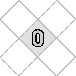
\includegraphics[scale=1]{0e0p/0e0p_rule_em_7077.pdf}} \hfill \vcenteredhbox{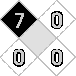
\includegraphics[scale=1]{0e0p/0e0p_rule_em_0007_0.pdf}}\vcenteredhbox{\color{black}{$\xrightarrow{\text{\clock{0}{1}}}$}} \vcenteredhbox{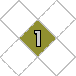
\includegraphics[scale=1]{0e0p/0e0p_rule_em_0007.pdf}} \hfill \vcenteredhbox{\patternimg{0.35}{rule_em_0070_0}}\vcenteredhbox{\color{black}{$\xrightarrow{\text{\clock{0}{1}}}$}} \vcenteredhbox{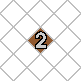
\includegraphics[scale=1]{0e0p/0e0p_rule_em_0070.pdf}} \hfill \vcenteredhbox{\patternimg{0.35}{rule_em_0077_0}}\vcenteredhbox{\color{black}{$\xrightarrow{\text{\clock{0}{1}}}$}} \vcenteredhbox{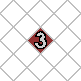
\includegraphics[scale=1]{0e0p/0e0p_rule_em_0077.pdf}} \\[1em]
	\vcenteredhbox{\patternimg{0.35}{rule_em_0700_0}}\vcenteredhbox{\color{black}{$\xrightarrow{\text{\clock{0}{1}}}$}} \vcenteredhbox{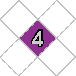
\includegraphics[scale=1]{0e0p/0e0p_rule_em_0700.pdf}} \hfill \vcenteredhbox{\patternimg{0.35}{rule_em_0707_0}}\vcenteredhbox{\color{black}{$\xrightarrow{\text{\clock{0}{1}}}$}} \vcenteredhbox{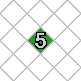
\includegraphics[scale=1]{0e0p/0e0p_rule_em_0707.pdf}} \hfill \vcenteredhbox{\patternimg{0.35}{rule_em_0770_0}}\vcenteredhbox{\color{black}{$\xrightarrow{\text{\clock{0}{1}}}$}} \vcenteredhbox{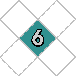
\includegraphics[scale=1]{0e0p/0e0p_rule_em_0770.pdf}} \hfill \vcenteredhbox{\patternimg{0.35}{rule_em_0777_0}}\vcenteredhbox{\color{black}{$\xrightarrow{\text{\clock{0}{1}}}$}} \vcenteredhbox{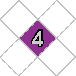
\includegraphics[scale=1]{0e0p/0e0p_rule_em_0700.pdf}} \\[1em]
	\vcenteredhbox{\patternimg{0.35}{rule_em_7000_0}}\vcenteredhbox{\color{black}{$\xrightarrow{\text{\clock{0}{1}}}$}} \vcenteredhbox{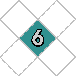
\includegraphics[scale=1]{0e0p/0e0p_rule_em_0770.pdf}} \hfill \vcenteredhbox{\patternimg{0.35}{rule_em_7007_0}}\vcenteredhbox{\color{black}{$\xrightarrow{\text{\clock{0}{1}}}$}} \vcenteredhbox{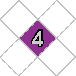
\includegraphics[scale=1]{0e0p/0e0p_rule_em_0700.pdf}} \hfill \vcenteredhbox{\patternimg{0.35}{rule_em_7070_0}}\vcenteredhbox{\color{black}{$\xrightarrow{\text{\clock{0}{1}}}$}} \vcenteredhbox{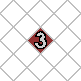
\includegraphics[scale=1]{0e0p/0e0p_rule_em_0077.pdf}} \hfill \vcenteredhbox{\patternimg{0.35}{rule_em_7077_0}}\vcenteredhbox{\color{black}{$\xrightarrow{\text{\clock{0}{1}}}$}} \vcenteredhbox{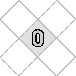
\includegraphics[scale=1]{0e0p/0e0p_rule_em_7077.pdf}} \\[1em]
	\vcenteredhbox{\patternimg{0.35}{rule_em_7700_0}}\vcenteredhbox{\color{black}{$\xrightarrow{\text{\clock{0}{1}}}$}} \vcenteredhbox{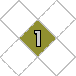
\includegraphics[scale=1]{0e0p/0e0p_rule_em_0007.pdf}} \hfill \vcenteredhbox{\patternimg{0.35}{rule_em_7707_0}}\vcenteredhbox{\color{black}{$\xrightarrow{\text{\clock{0}{1}}}$}} \vcenteredhbox{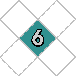
\includegraphics[scale=1]{0e0p/0e0p_rule_em_0770.pdf}} \hfill \vcenteredhbox{\patternimg{0.35}{rule_em_7770_0}}\vcenteredhbox{\color{black}{$\xrightarrow{\text{\clock{0}{1}}}$}} \vcenteredhbox{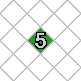
\includegraphics[scale=1]{0e0p/0e0p_rule_em_0707.pdf}} \hfill \vcenteredhbox{\patternimg{0.35}{rule_em_7777_0}}\vcenteredhbox{\color{black}{$\xrightarrow{\text{\clock{0}{1}}}$}} \vcenteredhbox{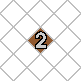
\includegraphics[scale=1]{0e0p/0e0p_rule_em_0070.pdf}}
	\caption{The rule for transitioning from even to odd generations in the $8$-state von-Neumann-neighborhood CA from Equation~\eqref{eq:0e0p_N_from_even}. The states $0$ and $7$ correspond to ``dead'' and ``alive'' in Life and are thus displayed in white and black, respectively. The states $1$, $2$, $3$, $4$, $5$, and $6$ are displayed in \bgbox{yellowback2}{yellow}, \bgbox{orangeback2}{orange}, \bgbox{redback}{red}, \bgbox{magentaback}{magenta}, \bgbox{greenpastel}{green}, and \bgbox{aquaback}{aqua}, respectively.}\label{fig:0e0p_rule_em}
\end{figure}

The reason for choosing these seemingly-random transition rules is that they lead to the function
\[
	\begin{pmatrix}
		a_{1,1} & a_{1,2} & a_{1,3} \\
		a_{2,1} & a_{2,2} & a_{2,3} \\
		a_{3,1} & a_{3,2} & a_{3,3}
	\end{pmatrix} \mapsto \begin{pmatrix}
		N\begin{pmatrix}
		a_{1,1} & a_{1,2} \\
		a_{2,1} & a_{2,2}
		\end{pmatrix} & N\begin{pmatrix}
		a_{1,2} & a_{1,3} \\
		a_{2,2} & a_{2,3}
		\end{pmatrix} \\
		N\begin{pmatrix}
		a_{2,1} & a_{2,2} \\
		a_{3,1} & a_{3,2}
		\end{pmatrix} & N\begin{pmatrix}
		a_{2,2} & a_{2,3} \\
		a_{3,2} & a_{3,3}
		\end{pmatrix}
	\end{pmatrix}
\]
from $\{0,7\}^9$ to $\{0,1,2,3,4,5,6\}^4$ being injective (i.e., each output of the function corresponds to a \emph{unique} input).\footnote{However, the choices we made in Equation~\eqref{eq:0e0p_N_from_even} (or equivalently, Figure~\ref{fig:0e0p_rule_em}) are not the only ones that lead to this function being injective. This collection of outputs, and many others, can be found by computer search---see Exercise~??.} That is, given any $2 \times 2$ arrangement of states $0$, $1$, $\ldots$, $6$, we can figure out which $3 \times 3$ arrangement of $0$ and $7$ states (if any) gave rise to it. We can thus define $N$ on inputs from $\{0,1,2,3,4,5,6\}^4$ so that Equation~\eqref{eq:0e0p_N_from_M} holds (i.e., the cellular automaton defined by $N$ emulates the cellular automaton defined by $M$ at half speed).

The resulting function $N$ is typically quite messy to write out in full detail (as it would just be an explicit list of how the $2^9 = 512$ possible arrangements of $2 \times 2$ grids of states $0$, $1$, $\ldots$, $6$ should evolve), even if the rule $M$ describes a relatively simple cellular automaton like Life. However, it can be constructed straightforwardly by a computer script,\footnote{One such script is available at \httpsurl{conwaylife.com/forums/viewtopic.php?p=38032}.} and the emulation of a glider in this way is illustrated in Figure~\ref{fig:0e0p_rule_em_glider}.

\begin{figure}[!htb]
	\centering
	\embedlink{0e0p_rule_em_glider}{\vcenteredhbox{\hphantom{${}\, \cdots$ \genarrow{1}}}\vcenteredhbox{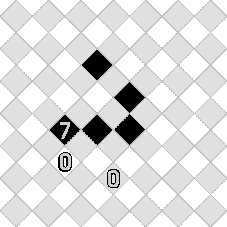
\includegraphics[scale=1]{0e0p/0e0p_glider_states0.pdf}} \vcenteredhbox{\genarrow{1}} \vcenteredhbox{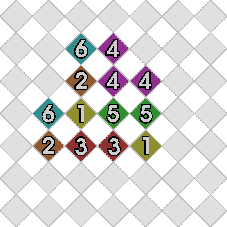
\includegraphics[scale=1]{0e0p/0e0p_glider_states.pdf}} \vcenteredhbox{\genarrow{1}} \vcenteredhbox{\patternimg{0.3}{0e0p_rule_em_glider_2}} \\[0.7em]
	\vcenteredhbox{$\cdots$ \genarrow{1}} \vcenteredhbox{\patternimg{0.3}{0e0p_rule_em_glider_3}} \vcenteredhbox{\genarrow{1}} \vcenteredhbox{\patternimg{0.3}{0e0p_rule_em_glider_4}} \vcenteredhbox{\genarrow{1}} \vcenteredhbox{\patternimg{0.3}{0e0p_rule_em_glider_5}} \\[0.7em] \vcenteredhbox{$\cdots$ \genarrow{1}} \vcenteredhbox{\patternimg{0.3}{0e0p_rule_em_glider_6}} \vcenteredhbox{\genarrow{1}} \vcenteredhbox{\patternimg{0.3}{0e0p_rule_em_glider_7}} \vcenteredhbox{\genarrow{1}} \vcenteredhbox{\patternimg{0.3}{0e0p_rule_em_glider_8}}}
	\caption{A glider from Life being emulated at half speed via an $8$-state cellular automaton using the von Neumann neighborhood (rotated by 45 degrees). Uses the same state coloring as in Figure~\ref{fig:0e0p_rule_em}, which describes the transitions from even to odd generations. The transitions from odd to even generations are encoded as an explicit list of which $2 \times 2$ arrangements of states $0$, $1$, $\ldots$, $6$ should lead to their central cell being born.}\label{fig:0e0p_rule_em_glider}
\end{figure}

The 0E0P metacell can be programmed to emulate any of the $8^{8^4-1}$ possible zero-preserving 8-state von-Neumann-neighborhood cellular automata in which every cell dies every generation (not just the ones that emulate one of the $2^{2^9-1}$ zero-preserving 2-state Moore-neighborhood CAs that we are actually interested in). It takes $2^{35}$ generations for the 0E0P metacell to run one generation of the 8-state rule (emulated at a 45-degree angle, as in the figures of this section), and therefore $2^{36}$ generations to emulate one generation of the corresponding 2-state Moore-neighborhood rule (in the usual orientation).


%%%%%%%%%%%%%%%%%%%%%%%%%%%%%%%%%%%
\section{Overview of the Metacell}\label{sec:0e0p_structure}
%%%%%%%%%%%%%%%%%%%%%%%%%%%%%%%%%%%

The 0E0P metacell works by using the single-channel glider synthesis techniques of Chapter~\ref{chp:universal_construction} to construct copies of itself in neighboring locations. It starts by constructing a copy to the southeast, northeast, northwest, and southwest (in that order, and only if no metacells are already present in those locations), and then it sends information about its current state to those neighboring metacells so that the proper rule is emulated.\index{single-channel synthesis}

In order to implement this behavior, the 0E0P metacell is made up of three components (see Figures~\ref{fig:0e0p_schematic} and~\ref{fig:0e0p_itself}), which are constructed by parent metacells one at a time:\smallskip

\begin{figure}[!htb]
	\centering
	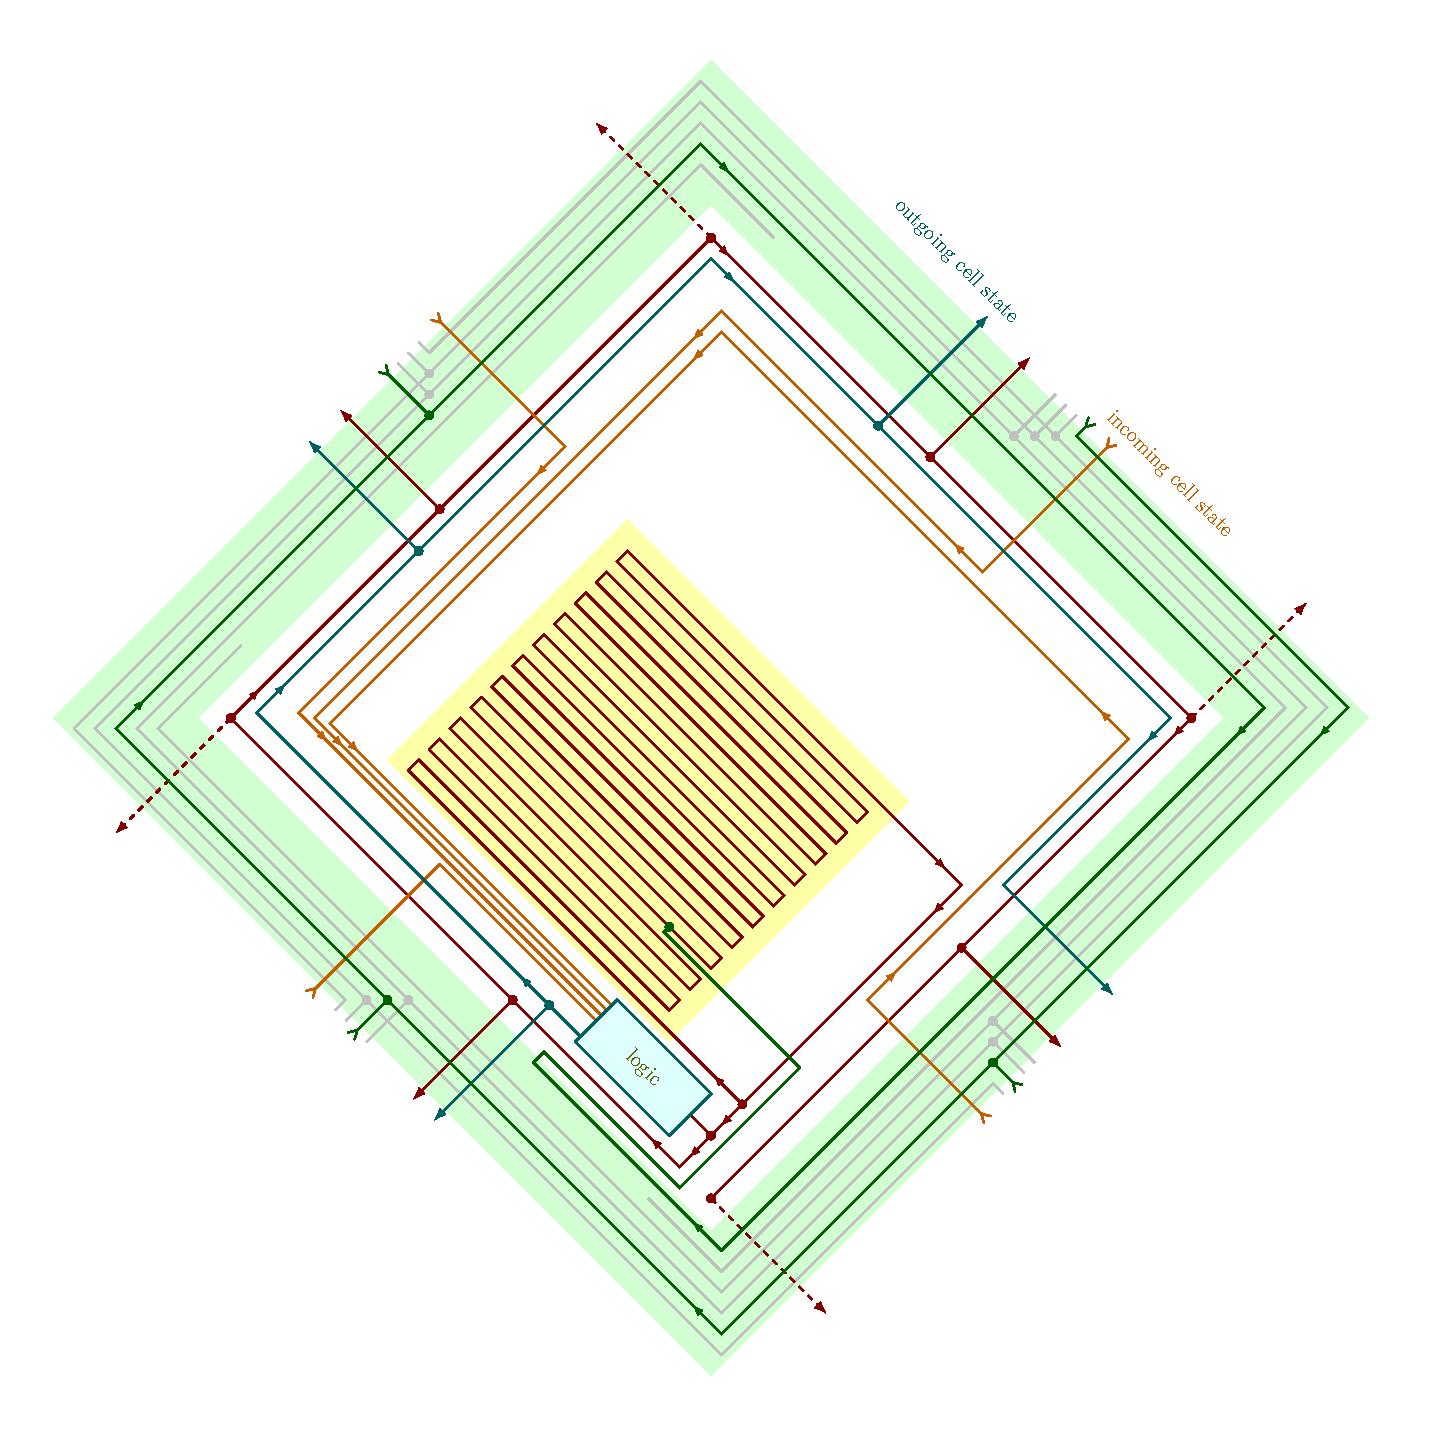
\includegraphics[width=\textwidth]{0e0p/0e0p_schematic.pdf}
	\caption{A schematic of the 0E0P metacell. The \textbf{nucleus}, highlighted in \bgbox{yellowback2}{yellow}, houses a single-channel glider sequence containing over 3~million gliders, which encode the rule being emulated as well as the construction of the 0E0P metacell itself. When the 0E0P is being constructed, its symmetrical outer \textbf{shell} (highlighted in \bgbox{greenpastel}{light green}) takes in the single-channel glider sequence from any of its neighboring parents (along the path displayed in \bgbox{greenback}{dark green}) and injects it into the nucleus. The unhighlighted region in the middle is the \textbf{kernel}, which contains an output path for a copy of the single-channel glider sequence (displayed in \bgbox{magentaback}{magenta}), as well as input and output paths along which parent metacells can tell child metacells what state they are in (displayed in \bgbox{orangeback2}{orange} and \bgbox{aquaback}{aqua}, respectively).}\label{fig:0e0p_schematic}
\end{figure}

\begin{figure}[!phtb]
	\centering
	\embedlink{0e0p}{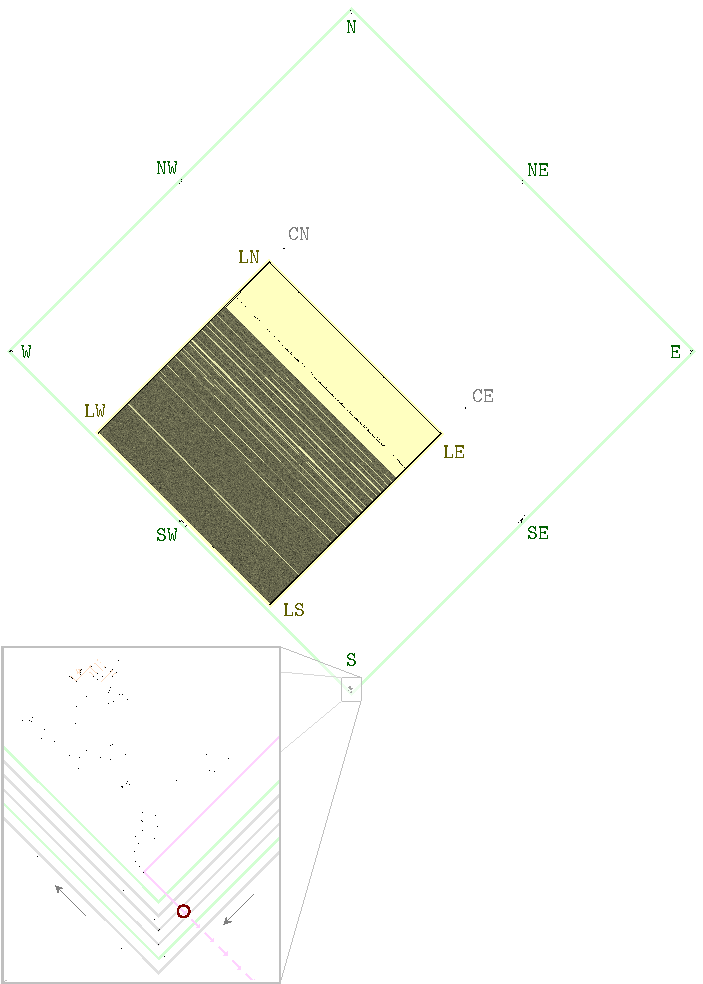
\includegraphics[width=\textwidth]{0e0p/0e0p.pdf}}	\caption{The 0E0P metacell itself, which implements the schematic of Figure~\ref{fig:0e0p_schematic}. It contains a significant amount of empty space between 15 points of interest. The shell (highlighted in \bgbox{greenpastel}{green}) goes through points \texttt{SW}, \texttt{W}, \texttt{NW}, \texttt{N}, \texttt{NE}, \texttt{E}, \texttt{SE}, and \texttt{S}, as do the points where the glider paths are reflected in the kernel. The logic circuitry is also located at point \texttt{S}, and an elbow block that is used to construct a new metacell to the southeast is circled in \bgbox{redback}{red}. The nucleus (highlighted in \bgbox{yellowback2}{yellow}) has corners at points \texttt{LW}, \texttt{LN}, \texttt{LE}, and \texttt{LS}. The point \texttt{INS} is used to insert gliders into the nucleus during construction. The points \texttt{CN} and \texttt{CE} are not displayed in the schematic of Figure~\ref{fig:0e0p_schematic}---they contain temporary circuitry that is used to construct the walls of the nucleus.}\label{fig:0e0p_itself}
\end{figure}

\begin{itemize}
	\item The outermost part is the \textbf{shell},\index{shell} which directs information about the states of neighboring metacells. It has exact 90-degree rotational symmetry, consisting of four spiral arms which propagate gliders inwards. Only one of these arms is actually used; the other four exist only to enforce the rotational symmetry.\smallskip
	
	\item Inside the shell is the \textbf{kernel},\index{kernel} which does not have any symmetry constraints. The south corner of the kernel contains a clock gun for regulating the metacell's lifecycle and logic circuitry for computing the state of the metacell based on the states of its four neighboring cells. The kernel also contains an output path, shown in magenta in Figure~\ref{fig:0e0p_schematic}, which can connect to one of the four construction arms (dashed) or to the input shell of one of the four neighbours.\smallskip
	
	\item At its center is the largest region of the metacell: its \textbf{nucleus},\index{nucleus} which is a huge glider loop with a period of exactly $2^{29}$. It is populated by over three million gliders, consisting of a complete single-channel glider synthesis of the 0E0P metacell, as well as a state lookup table that encodes the rule that the metacell is emulating.\smallskip
\end{itemize}

We describe how these three components of the metacell function throughout its lifecycle in more detail in the next three sections, and we then talk about how they are constructed by parent metacells in Section~\ref{sec:0e0p_construction}. Due to the complexity and size of the 0E0P metacell, it is extremely important that the reader does not just read through the next few sections, but also explores the metacell's different components as we describe them via Life simulation software.\footnote{Unfortunately, no Life simulation software is currently fast enough to run the entire 0E0P metacell ``quickly''. However, bits and pieces of it can be evolved to see how they behave, and numerous snapshots that show the metacell's state at different timestamps are provided in Section~\ref{sec:0e0p_timeline} and at \httpsurl{conwaylife.com/book/patterns.php?p=0e0p}.}


%%%%%%%%%%%%%%%%%%%%%%%%%%%%%%%%%%%
\section{The Shell and Lane-Switching Circuitry}\label{sec:0e0p_structure_shell}\index{shell}
%%%%%%%%%%%%%%%%%%%%%%%%%%%%%%%%%%%

The rotationally symmetric shell that makes up the outermost edges of the 0E0P metacell is the simplest of its three components. At each of the locations marked \texttt{SW}, \texttt{NW}, \texttt{NE}, and \texttt{SE} in Figure~\ref{fig:0e0p_itself}, there are four recipe input lanes (in green and grey in Figure~\ref{fig:0e0p_schematic}). However, only one of those four lanes is ever actually used (in green)---the one that connects to the recipe output lane coming in from the kernel of the neighboring metacell (in solid magenta), if it exists.\footnote{This design is similar to that of a circuit on a motherboard---you can think of each side of the 0E0P metacell as having 8 ``pins'' (4 inputs pins and 4 output pins) that connect to the 8 pins of neighboring metacells.} The remaining input lanes (in grey) are unused, and only exist to enforce the shell's fourfold rotational symmetry.

After the metacell has been constructed, these input lanes read in a copy of the 0E0P's single-channel construction recipe and state lookup table from its neighbors. That (extremely long) sequence of gliders revolves clockwise all the way around the spiral arm of the shell, until it is finally injected into the nucleus (at the location called \texttt{INS} in Figure~\ref{fig:0e0p_itself}) at the 0E0P's center.

To make sure that just one copy of the single-channel glider sequence is allowed to enter the shell, regardless of how many neighbors try to send in that glider sequence, the 0E0P metacell strategically deletes part of its own circuitry after the nucleus is populated (as well as at numerous other times throughout its lifecycle). By using a stray glider to delete a single block from a syringe, as demonstrated in Figure~\ref{fig:syringe_delete_block}, the 0E0P can change a syringe-based-reflector into a device that simply eats a glider stream. Another stray glider could also be used to destroy the syringe's eater~2, thus unblocking the stream as demonstrated in Figure~\ref{fig:syringe_delete_eater}, if desired. Extra stray gliders like these ones are provided by the metacell's control clock gun, which we discuss in the upcoming Section~\ref{sec:0e0p_structure_clock}.

\begin{figure}[!htb]
	\centering
	\begin{subfigure}{.535\textwidth}
		\centering
		\embedlink{syringe_path_changer}{\vcenteredhbox{\patternimg{0.12}{syringe_delete_block}} \vcenteredhbox{\genarrow{120}} \vcenteredhbox{\patternimg{0.12}{syringe_delete_block_1}}}
		\caption{A single glider coming in from the southwest destroys a block, thus ``shutting off'' the syringe-based reflector.}
		\label{fig:syringe_delete_block}
	\end{subfigure} \hfill \begin{subfigure}{.435\textwidth}
		\centering
		\patternlink{syringe_path_changer}{\vcenteredhbox{\patternimg{0.12}{syringe_delete_eater}} \vcenteredhbox{\genarrow{120}} \vcenteredhbox{\patternimg{0.12}{syringe_delete_eater_1}}}
		\caption{A glider coming in from the northeast destroys the eater~2, thus unblocking the glider stream.}
		\label{fig:syringe_delete_eater}
	\end{subfigure}
	\caption{Some ways of deleting pieces of a syringe (displayed in \bgbox{redback}{red}) so as to change the path of a glider stream.}\label{fig:syringe_path_changer}
\end{figure}


%%%%%%%%%%%%%%%%%%%%%%%%%%%%%%%%%%%
\section{The Kernel}\label{sec:0e0p_structure_kernel}\index{kernel}
%%%%%%%%%%%%%%%%%%%%%%%%%%%%%%%%%%%

The asymmetric kernel contains the paths that are used to feed the 0E0P's single-channel recipe into its neighbors (in magenta in Figure~\ref{fig:0e0p_schematic}). Along these paths, gliders spiral clockwise-and-outwards, and then bypass the shell and do one of two things: go into a construction lane (in dashed magenta) to construct a neighboring metacell, or go into a recipe output lane (in solid magenta) that connects to a recipe input lane of an already-constructed neighboring metacell.

One important aspect of how the recipe output and input lanes of neighboring metacells connect to each other is that, irrespective of the orientation of the neighbors that are communicating, the single-channel glider sequence performs exactly 6 spiral quarter-turns to get from the south corner of the parent metacell to the south corner of the child metacell. This is how child metacells always end up in the correct phase and orientation after they are constructed. There are also some trombone slides of different lengths on different edges of the kernel, designed to compensate for the ``Olympic running track'' effect---the fact that outer lanes of the spiral are slightly longer than inner lanes. These trombone slides ensure that the communication time from the parent to each of the four children is exactly the same.

In order to control which recipe output lane or construction lane the single-channel glider sequence enters, the 0E0P periodically destroys some of the kernel's Snarks. We saw one method of doing this back in Figure~\ref{fig:snark_seeded_destroy}---a single glider can be used to destroy a Snark (with the help of 3 extra pre-placed still lifes). The 0E0P metacell makes use of Snark-destroying reactions like this one\footnote{But not \emph{exactly} this one---see Exercise~\ref{exer:0e0p_snark_destroyer}.} so as to redirect copies of its single-channel glider sequence to eight different locations over the course of its lifespan. In order,\footnote{The single-channel glider sequence really does have to be sent along these $8$ paths one after another. If we just used glider duplicators to send it along all $8$ paths at the same time, there could be unwanted collisions when constructing child metacells (e.g., if two parent metacells tried to create a child in the same location at the same time).} they are:\smallskip

\begin{itemize}
	\item[1)] Along the southeast construction lane (in dashed magenta in Figure~\ref{fig:0e0p_schematic}), to construct the child metacell to the southeast.\smallskip
	
	\item[2)] Along the southeast recipe output lane (in solid magenta), to copy the glider sequence into the (now constructed) southeast child's nucleus.\smallskip
	
	\item[3)] Along the northeast construction lane (in dashed magenta), to construct the child metacell to the northeast.\smallskip
	
	\item[4) -- 8)] Along the northeast recipe output lane, then the northwest construction lane, and so on counterclockwise.
\end{itemize}


%%%%%%%%%%%%%%%%%%%%%%%%%%%%%%%%%%%
\subsection{The Control Clock Gun}\label{sec:0e0p_structure_clock}\index{clock!gun}\index{control clock gun}
%%%%%%%%%%%%%%%%%%%%%%%%%%%%%%%%%%%

The lane-switching mechanisms described earlier are implemented by a \textbf{control clock gun} that is located at the top-left corner of the ``\texttt{logic}'' component in Figures~\ref{fig:0e0p_schematic} and~\ref{fig:0e0p_itself}.\footnote{There are actually four clock guns in the 0E0P metacell. This ``control'' clock gun is active for the entirety of the metacell's lifecycle, while the other three are all temporary.} This gun sends out a single glider every $2^{29}$ generations, thus matching exactly the period of the glider loop contained in the nucleus. It is made up of a p256 gun attached to a sequence of $21$ semi-Snarks, much like the clock gun of Figure~\ref{fig:p2to_the_20_gun} that was used by Chapter~\ref{chp:universal_computation}'s universal computer (though that gun used quadri-Snarks instead).\footnote{The 0E0P's clock guns use the color-changing semi-Snark of Figure~\ref{fig:cc_semi_snark}, since it is Spartan and is thus easier to construct via a single-channel glider recipe than quadri-Snarks.}\index{semi-Snark}\index{Spartan}

The gliders that are released by the control clock gun travel through sequences of one-time turners and splitters that are interspersed throughout the rest of the 0E0P's circuitry, so as to trigger the appropriate lane-switching mechanisms at each step of its lifecycle. This method is illustrated at a much smaller scale in Figure~\ref{fig:clock_path_switcher}, where a clock gun is used to change what happens to the path of a single-channel glider sequence three times.

\begin{figure}[!htb]
	\centering
	\embedlink{clock_path_switcher}{\vcenteredhbox{\hphantom{${}\ {}$ \genarrow{20}}}\vcenteredhbox{\patternimg{0.105}{clock_path_switcher_0}} \vcenteredhbox{\color{black}{$\xrightarrow{\text{\clock{4}{45} $2^{12}$}}$}} \vcenteredhbox{\patternimg{0.105}{clock_path_switcher_1}} \\[0.7em]
	\vcenteredhbox{\color{black}{$\xrightarrow{\text{\clock{4}{45} $2^{12}$}}$}} \vcenteredhbox{\patternimg{0.105}{clock_path_switcher_2}} \vcenteredhbox{\color{black}{$\xrightarrow{\text{\clock{4}{45} $2^{12}$}}$}} \vcenteredhbox{\patternimg{0.105}{clock_path_switcher_3}}}
	\caption{A period~$2^{12} = 4{\thousep}096$ clock gun (highlighted in \bgbox{aquaback}{aqua}) using one-time turners and the reactions from Figures~\ref{fig:snark_seeded_destroy} and~\ref{fig:syringe_path_changer} to change the path of the single-channel glider stream coming from the northwest. Initially, that stream is reflected to the northeast, but the first glider from the clock gun blocks the reflector. Its second glider unblocks it and redirects the stream to the southwest via a Snark. Its third glider destroys the Snark, so the stream passes straight through to the southeast.}\label{fig:clock_path_switcher}
\end{figure}

In the actual 0E0P, the control clock gun's output is redirected many more times than this, and the one-time circuitry involved is much more complex. Furthermore, it also has a period~$2^{25}$ output lane that spends most of its time blocked, but is periodically unblocked so that it can send out a glider with different timing than the main period~$2^{29}$ output lane. Jump ahead to Figure~\ref{fig:0e0p_clock_gun_full} to see what the period~$2^{29}$ output lane actually looks like.


%%%%%%%%%%%%%%%%%%%%%%%%%%%%%%%%%%%
\subsection{Logic Circuitry and State Computation}\label{sec:0e0p_structure_logic}
%%%%%%%%%%%%%%%%%%%%%%%%%%%%%%%%%%%

The kernel also contains, at its southern corner (i.e., the location called \texttt{S} in Figure~\ref{fig:0e0p_itself}), the logic circuitry that is used to compute the metacell's state from the states of its four neighboring parents. Metacells' states are transmitted via sequences of gliders, and are stored via \emph{absences} of blocks, as follows:\smallskip

\begin{itemize}
	\item \textbf{Transmission}: When a parent metacell sends its state to its children, it does so via a sequence of $0$ or $2$--$8$ gliders, representing state $0$ or $1$--$7$, respectively.\footnote{That is, it represents its state in unary, but with an extra glider if it is in any non-zero state.}\index{unary}\smallskip
	
	\item \textbf{Temporary storage}: When children receive their parents' states, the first glider (if it exists) is used to unblock their control clock gun, while the remaining $1$--$7$ gliders destroy $1$--$7$ blocks. The children thus temporarily store their parents' states in the \emph{absence} of those blocks.\smallskip
	
	\item \textbf{Internal transmission}: After a child computes its state from its parents, it initially appears as a unary sequence of $0$--$7$ gliders. One-time circuitry is used to duplicate one of those gliders (if they exist), resulting in a sequence of $0$ or $2$--$8$ gliders.\smallskip
	
	\item \textbf{Long-term storage}: Those $0$ or $2$--$8$ gliders are aimed at a sequence of $8$ blocks at the westernmost edge of the child's ``\texttt{S}'' corner (see the upcoming Figure~\ref{fig:0e0p_timeline_8054294330} for the precise location). Its state is thus stored in the \emph{absence} of those blocks, with state $0$ corresponding to $8$ blocks and state $1 \leq s \leq 7$ corresponding to $7 - s$ blocks.\smallskip
\end{itemize}

To compute its state from those of its parents, a child metacell uses a lookup table: a collection of $8^4 - 1 = 4{\thousep}095$ sequences of $0$--$7$ gliders each, arranged in $1{\thousep}024$-generation chunks, specifying what the new state should be given any possible combination of not-all-zero parent states. This lookup table is stored in the nucleus, and we can use the one-time switching techniques of Section~\ref{sec:0e0p_structure_shell} to extract a single $1{\thousep}024$-generation chunk from it. To extract the \emph{correct} chunk, however, we have to delay those one-time switching operations to the correct moment in time, based on the absence of the blocks representing parent metacells' states. To this end, the child metacell uses a \textbf{state-lookup clock gun}\index{state-lookup clock gun} like the one illustrated in Figure~\ref{fig:state_lookup_clock_gun}.\footnote{However, the gun illustrated here only plucks out a single glider. To have it pluck out up to $7$ gliders, its one-time circuitry has to be modified slightly (see Exercise~\ref{exer:0e0p_state_lookup_wider}).}

\begin{figure}[!htb]
	\centering
	\embedlink{state_lookup_clock_gun}{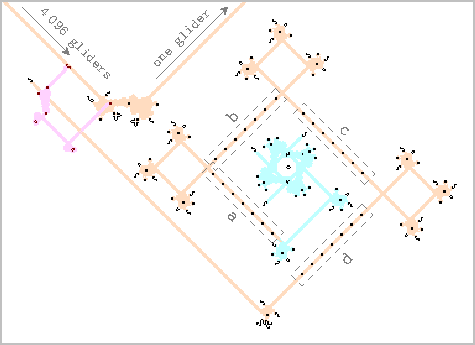
\includegraphics[width=\textwidth]{0e0p/state_lookup_clock_gun.pdf}}
	\caption{A period~$1024$ clock gun (highlighted in \bgbox{aquaback}{aqua}) that has blocks along its path, delaying its first output glider. If there are $a$ blocks along the southwest edge, $b$ along the northwest edge, $c$ along the northeast edge, and $d$ along the southeast edge, then the clock gun's first escaping glider is produced by the Herschel that is present at generation $1024(a + 8b + 64c + 512d)$. That glider hits one-time circuitry (highlighted in \bgbox{magentaback}{magenta}) that unblocks and quickly re-blocks a glider stream, allowing its $(1 + a + 8b + 64c + 512d)$-th glider to escape.}
	\label{fig:state_lookup_clock_gun}
\end{figure}

This mechanism works by placing blocks and semi-Snarks along a period~$1{\thousep}024$ clock gun's output path: each block destroys a single glider, thus delaying the glider that will trigger the one-time switching circuitry. However, if a semi-Snark is placed between the clock gun and the block, then \emph{two} gliders will be destroyed: one by the block and then another one by the semi-Snark. More generally, placing $k$ semi-Snarks between the clock gun and the block results in the clock gun's first $2^k$ output gliders being destroyed.

It follows that if we place $0 \leq a,b,c,d \leq 7$ blocks along the gun's output lane, with $3$ semi-Snarks between each of those groups of blocks, then
\[
	a + (2^3)b + (2^6)c + (2^9)d = a + 8b + 64c + 512d
\]
gliders will be absorbed before the first one escapes.\footnote{This is similar to the method that we saw in Figure~\ref{fig:block_18_gliders} for blocking a specific number of gliders via semi-Snarks, but is easier to synthesize and configure.} That first escaping glider then hits one-time circuitry that unblocks a copy of the state lookup table, re-blocks it just over $900$ generations later,\footnote{The sequences of $0$--$7$ gliders in the state lookup table are separated by $1{\thousep}024$ generations (the period of the state-lookup clock gun). However, roughly $10\%$ of that space is unusable and must remain empty so that it does not interfere with the unblocking and re-blocking reactions.} and causes the state-lookup clock gun to self-destruct.


%%%%%%%%%%%%%%%%%%%%%%%%%%%%%%%%%%%
\section{The Nucleus}\label{sec:0e0p_structure_nucleus}\index{nucleus}
%%%%%%%%%%%%%%%%%%%%%%%%%%%%%%%%%%%

The 0E0P metacell's nucleus is a massive boustrophedonic loop\footnote{That is, a loop made up of numerous antiparallel lanes.} that houses roughly $3.6$~million gliders. Its corners are located at the positions marked \texttt{LS}, \texttt{LW}, \texttt{LN}, and \texttt{LE} in Figure~\ref{fig:0e0p_itself}, and its walls between \texttt{LW} and \texttt{LN}, and between \texttt{LE} and \texttt{LS}, are each made up of $2^{10} = 1{\thousep}024$ two-Snark (i.e., $180$-degree) reflectors. The walls of the nucleus are separated by roughly $2^{16} = 65{\thousep}536$ full diagonals, so that altogether it takes a glider exactly
\[
	2^{16} \times 2^{10} \times 4 \times 2 = 2^{29}
\]
generations to loop through it.

However, a small fraction of these $2^{29}$ generations are spent with gliders outside of the nucleus. After cycling through the nucleus's Snark walls, gliders are directed southeast past the corner at \texttt{LE} to the locations marked \texttt{SE}, then \texttt{S}, and then back into the nucleus at \texttt{LW}. The important part of this process is the time spent with the logic circuitry at \texttt{S}, where the contents of the nucleus can be duplicated and redirected so as to construct a child metacell, or the metacell's state can be extracted from a copy of the nucleus's lookup table.

On the other hand, when a metacell's nucleus is being populated for the first time, gliders are instead inserted into it at the location marked \texttt{INS} in Figure~\ref{fig:0e0p_itself}, which is several rows ahead of the start of the loop at \texttt{LW}. This ``head start'' compensates for the fact that this first copy of the nucleus's contents is coming from farther away---the metacell that constructed it---and ensures that the memory loops of the parent and child metacells end up in exactly the same phase.


%%%%%%%%%%%%%%%%%%%%%%
\section{Construction and Self-Destruction}\label{sec:0e0p_construction}\index{single-channel synthesis}
%%%%%%%%%%%%%%%%%%%%%%

Copies of the 0E0P metacell construct each other via the single-channel glider synthesis techniques of Chapter~\ref{chp:universal_construction}. Indeed, the vast majority of the contents of the nucleus are a single-channel glider recipe that carries out this task. For the most part, this construction is straightforward, with long-distance elbow pushes via Corderships\index{Cordership} (as we described back in Section~\ref{sec:medium_demonoid}) being one of its most complicated pieces.\footnote{The 0E0P metacell uses 3-engine Corderships for these long-distance elbow pushes, since the single-channel recipe for the 2-engine Cordership from Figure~\ref{fig:2_engine_cordership_seed} and Appendix~\ref{sec:appendix_cordership_maker} was not known at the time of its completion in 2018. The faster crab-based elbow-pushing method of Section~\ref{sec:fast_demonoid_elbow_carry} was also not yet known.}

However, there are two particular problems that arise when trying to construct child metacells that are worth clarifying and focusing on:\smallskip

\begin{itemize}
	\item \textbf{Child orientation}: We need all metacells to be constructed in the same orientation, regardless of whether they are being constructed by a parent to the northwest, southwest, southeast, or northeast. This is ensured by first building the child's shell\index{shell} (which is impossible to get wrong, since it is rotationally symmetric) and then sending the remainder of the single-channel recipe through the correct recipe input lane so as to build the kernel in the correct orientation. If we'd counterfactually sent the recipe down one of the other three input lanes, it would end up in a different one of the four spiral arms and the resulting metacell would be constructed in the wrong orientation.\smallskip
	
	\item \textbf{Nucleus walls}: Each of the 180-degree reflectors along the walls of the nucleus is quite expensive, requiring somewhere between $2^{20}$ and $2^{21}$ generations for a single-channel glider recipe to construct. It follows that a recipe for the $2 \times 2^{10} = 2{\thousep}048$ reflectors used by the nucleus would be more than $2 \times 2^{10} \times 2^{20} = 2^{31}$ generations long, and would thus not fit inside the period $2^{29}$ nucleus.
	
	We could try getting around this problem by adding more rows to the nucleus, but this does not work: adding another $180$-degree reflector on each of its northwest and southeast sides increases the length of the glider sequence that it can store by approximately $2^{19}$ generations, but increases the length of its construction recipe by more than $2 \times 2^{20}$ generations. It thus becomes necessary to increase the \emph{width} of each row of the nucleus so that it takes $2^{21}$ generation for gliders to travel from one wall to the other, making it eight times as wide as in the actual 0E0P: $2^{19} = 524{\thousep}288$ full diagonals instead of $2^{16} = 65{\thousep}536$.\smallskip
\end{itemize}

In order to avoid the aforementioned factor-of-eight width increase, the 0E0P metacell only stores a construction recipe for a single 180-degree reflector, and builds temporary circuitry (which we call a \textbf{subroutine loop})\index{subroutine loop} that allows that reflector-building recipe to be copied and used over and over again. Due to parity constraints, the reflectors along the northwest and southeast walls have a different shape, so it is actually necessary to have \emph{two} period~$2^{21}$ subroutines: one for the northwest wall, and one for the southeast wall. In the terminology of Figure~\ref{fig:0e0p_itself}, these subroutine loops are located at points \texttt{CN} and \texttt{CE}, respectively.

These subroutine loops reduce the problem of constructing an immense ($2^{29}$-generation) glider loop to the problem of constructing two smaller ($2^{21}$-generation) subroutine loops. Fortunately, the period~$2^{21}$ loops are small enough that they can be built without any special tricks, along with the rest of the metacell's kernel. Each subroutine loop is each equipped with its own clock gun that halts the subroutine after it has run for exactly 256 iterations. and built $256 \times 4 = 1{\thousep}024$ reflectors.
% Figure like Stage 0 (yellow) somewhere in here.

Destruction next.
% Talk about destruction by still lifes just like the speed demonoid here
% say the Snark and scorbie splitter are most complicated pieces (is it actually scorbie splitter in 0E0P?). Then show semi-Snark destruction picture here?

% EXercise: Explain why 4 fanouts in CE and CN construction
% Solution: to construct 8 times faster (since we want the nucleus 8 times skinnier). 2 times faster already gotten by doing both sides in parallel instead of sequential.


%%%%%%%%%%%%%%%%%%%%%%
\section{A Complete Metageneration}\label{sec:0e0p_timeline}\index{metageneration}
%%%%%%%%%%%%%%%%%%%%%%

So far, we have described how the 0E0P metacell works at a fairly high level: every $2^{29}$ generations, the clock gun fires a glider that potentially changes what happens throughout the metacell. Some of these gliders direct the single-channel glider sequence from the nucleus to start constructing a neighboring metacell, some of them trigger a signal that sends the metacell's state to its children, and some of them trigger the self-destruction of the entire metacell.

If we break the $2^{35}$-generation lifecycle of the metacell down into $2^6 = 64$ ``stages'' of $2^{29}$ generations each, then they behave roughly as follows:\smallskip

\begin{itemize}
	\item Stage 0: The metacell constructs its southeast neighbor.\smallskip
	
	\item Stage 1: It duplicates the contents of its nucleus into that of the southeast neighbor.\smallskip
	
	\item Stage 2: It constructs its northeast neighbor.\smallskip
	
	\item Stage 3: It duplicates the contents of its nucleus into that of the northeast neighbor.\smallskip
	
	\item Stages 4--7: Repeat stages 0--3 for the northwest and then southwest neighbors.\smallskip
	
	\item Stages 8--11: Do nothing (just spend some time ``looking like a cell'').\smallskip
	
	\item Stage 12: Minor cleanup (erase a single Snark).\smallskip
	
	\item Stage 13: Empty the single-channel glider stream out of the metacell's nucleus.\smallskip
	
	\item Stage 14: The parent metacell sends its state to all four of its children.\smallskip
	
	\item Stage 15: The parent metacell self-destructs while the child metacells compute their states.\smallskip
	
	\item Stages 16--63: Child metacells either self-destruct (if their state is $0$) or do nothing (if their state is non-zero, they just spend time ``looking like a cell'').\footnote{This wait time is only present so that patterns made up of metacells spend a decent amount of time looking, from a distance, like the patterns that they are emulating. When building the 0E0P metacell, Goucher underestimated how long it would take to run in Life simulation software---it could be modified to run $4$ times as quickly by removing this wait time.}\smallskip
\end{itemize}

These stages are each triggered by one-time circuitry that is placed along the period $2^{29}$ output lane of clock gun, as illustrated in Figure~\ref{fig:0e0p_clock_gun_full}. We now describe what happens throughout the 0E0P metacell's lifecycle in much more specific detail, and highlight key timestamps where interesting things happen or change in its circuitry.

\begin{figure}[!htbp]
	\centering
	\embedlink{clock_gun_full_small}{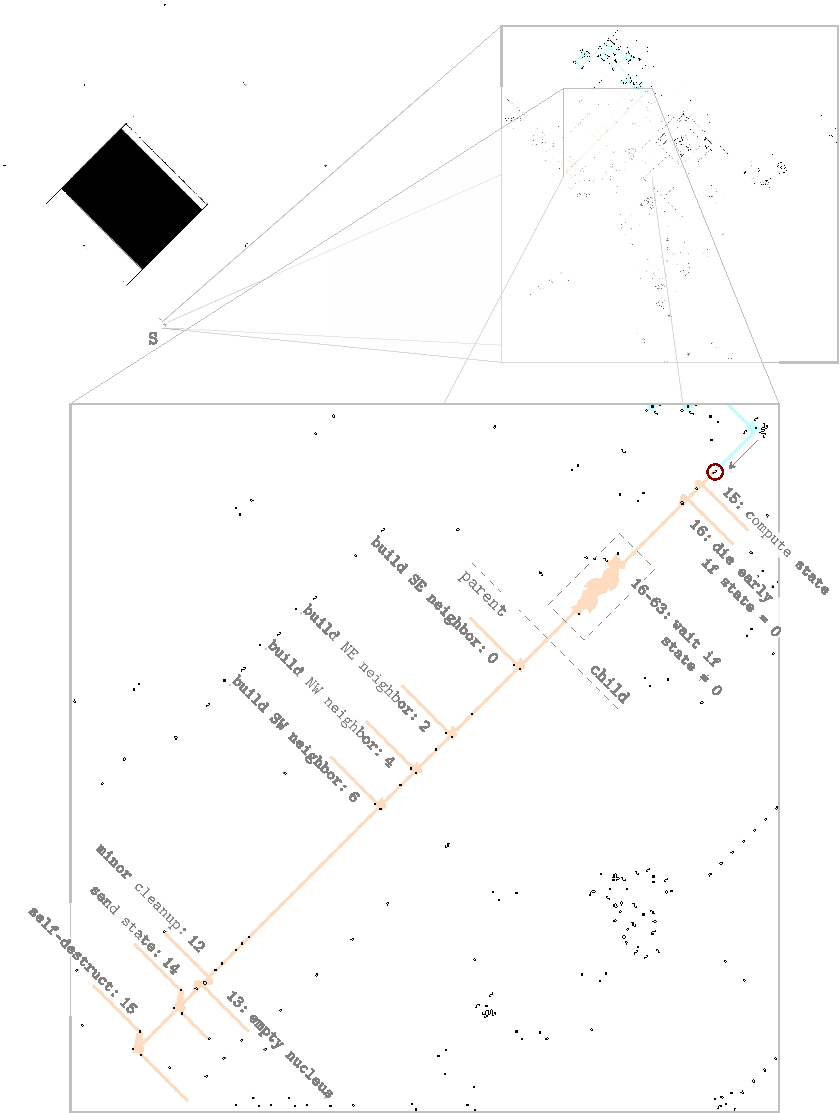
\includegraphics[width=1\textwidth]{0e0p/clock_gun_full.pdf}}
	\caption{One-time circuitry is used to direct the output of the metacell's period~$2^{29}$ control clock gun (highlighted in \bgbox{aquaback}{aqua}) to trigger various stages of its lifecycle. The stages begin when the eater~1 circled in \bgbox{redback}{red} is removed. After that, the metacell computes its state and either dies (if its state is 0) or does nothing for a long time (if its state is non-zero). Stages $16$--$63$, where child cells do nothing, are implemented by a slow salvo seed along the output lane that eats $48$ gliders before being destroyed. It then begins acting as a parent metacell rather than as a child: it starts building its own children in stage~0, it starts dying off in stage~12, and it sends its state to its children in stage 14.}
	\label{fig:0e0p_clock_gun_full}
\end{figure}

% To convert a timestamp from here to a timestamp from 0e0p_timeline.mc, add 105036424
% T = 0 is generation 178824 of RRO_backup_100487.
% To get generation t, look in rrocell_X, where X = 100487 + floor((t+178824)/262144) at generation (t+178824) mod 262144

% Rule table goes in before anything else (at LW?). Copy of DNA goes in through Area 51.


%%%%%%%%%%%%%%%%%%%%%%
\subsection{The First $\mathbf{0.26 \times 2^{29}}$ Generations: Construction of the Southeast Child's Shell}\label{sec:0e0p_timeline_shell}
%%%%%%%%%%%%%%%%%%%%%%

We start with an 0E0P metacell that is beginning to act like a parent: it is at the start of stage~$0$, and is ready to start constructing its children. We say that generation $t = 0$ is the one displayed in Figure~\ref{fig:0e0p_timeline_0}: the metacell has a Herschel in its clock gun that will create a glider that escapes past all of the semi-Snarks, hits a one-time turner on the period~$2^{29}$ output lane, and is redirected so as to remove an eater~1 that is blocking the clock gun's period $2^{25}$ output lane.

\begin{figure}[!htb]
	\centering
	\embedlink{0e0p_timeline_0_small}{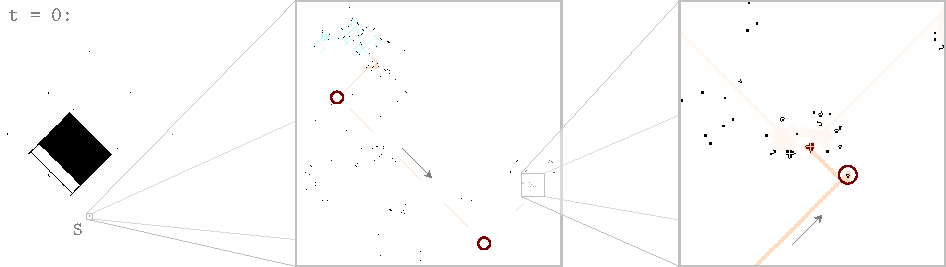
\includegraphics[width=1\textwidth]{0e0p/0e0p_timeline_0.pdf}}
	\caption{A Herschel in the parent metacell's clock gun (highlighted in \bgbox{aquaback}{aqua}) is about to create a glider that will make it out of its period $2^{29}$ branch. That glider will destroy an eater (circled in \bgbox{redback}{red}) so that the next glider can escape along that path $2^{25}$ generations later.}
	\label{fig:0e0p_timeline_0}
\end{figure}

A glider escapes via that new path $2^{25}$ generations later, at $t = 33{\thousep}554{\thousep}432 = 0.0625 \times 2^{29}$, and removes an eater~2 from a syringe (see Figure~\ref{fig:0e0p_timeline_33554432}). This unblocks a copy of the single-channel glider recipe, which now spirals outward through the kernel until it reaches the construction elbow at the metacell's south corner. That construction elbow is then pushed southeast, and is used to begin constructing the southeast child metacell's symmetric shell.

\begin{figure}[!htb]
	\centering
	\embedlink{0e0p_timeline_33554432_small}{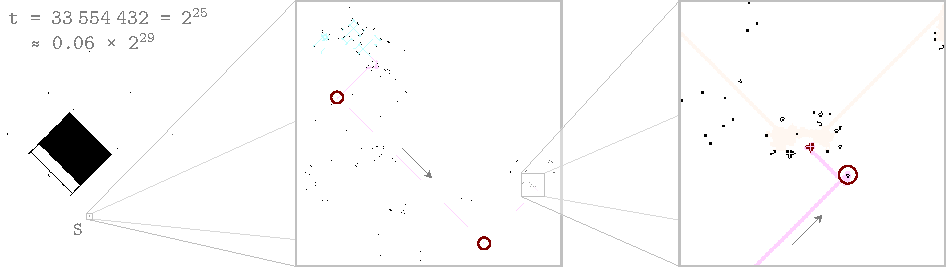
\includegraphics[width=1\textwidth]{0e0p/0e0p_timeline_33554432.pdf}}
	\caption{A Herschel in the parent metacell's clock gun (highlighted in \bgbox{aquaback}{aqua}) is about to create a glider that will escape via the path that was cleared in Figure~\ref{fig:0e0p_timeline_0}. It will use some one-time turners (circled in \bgbox{redback}{red}) and then destroy an eater~2 from a syringe, which will allow a copy of the single-channel glider recipe to escape from the nucleus and start constructing the southeast child metacell, starting with its shell.}
	\label{fig:0e0p_timeline_33554432}
\end{figure}

Construction of the child's symmetric shell continues in several stages. A stage often begins with the construction of a Cordership, followed by a slow salvo to shoot down the Cordership once it has traveled the right distance and turn it into a new target ``hand'' block at the correct location. Another slow salvo recipe then follows, to build whatever is needed at the location of the new hand block. There are many visible gaps in the 0E0P's single-channel recipe, and most of them correspond to the flight time of a Cordership, while the recipe waits to shoot it down after it has travelled the right distance.

The first such Cordership launch happens at generation $t = 50{\thousep}921{\thousep}682 \approx 0.0948 \times 2^{29}$ (see Figure~\ref{fig:0e0p_timeline_50921682}), where a Cordership is constructed at the child's south corner and is launched to its east corner.

\begin{figure}[!htb]
	\centering
	\embedlink{0e0p_timeline_50921682_small}{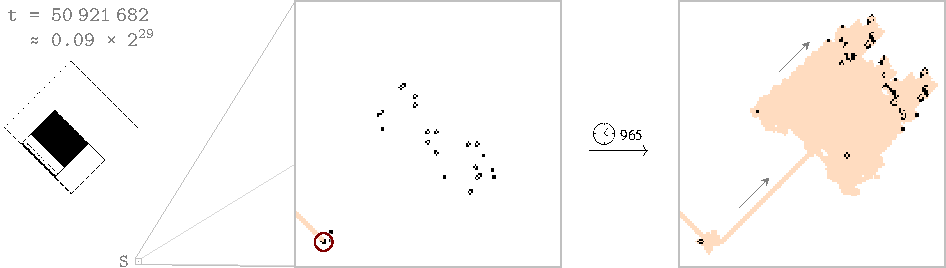
\includegraphics[width=1\textwidth]{0e0p/0e0p_timeline_50921682.pdf}}
	\caption{A glider (circled in \bgbox{redback}{red}) at the south corner of the child metacell's shell, about to synthesize a Cordership that does a long-distance elbow push to its east corner.}
	\label{fig:0e0p_timeline_50921682}
\end{figure}

By generation $t = 139{\thousep}291{\thousep}154 \approx 0.2594 \times 2^{29}$, construction of the final south corner of the symmetric shell is just about complete---the final construction glider has been produced, and a long-range backwards elbow move (\textbf{LRBEM})\index{LRBEM} recipe is processed immediately after this. At $t = 140{\thousep}354{\thousep}185 \approx 0.2614 \times 2^{29}$, the return glider from this LRBEM recipe has made a new elbow, and the single-channel recipe then shoots a single glider sideways from the new elbow position (at $t = 140{\thousep}355{\thousep}701$), removes the elbow (at $t = 140{\thousep}356{\thousep}370$), and then uses five gliders to clean up some leftover junk from the LRBEM (at $t = 140{\thousep}880{\thousep}132$), far away in the northeast corner.\footnote{This out-of-order cleanup is just the way that slsparse automatically compiled these LRBEMs in 2018. There are more efficient recipes known now.}

That single extra stray glider that was shot sideways by the temporary elbow will be used shortly to trigger construction of the southeast child metacell's kernel.


%%%%%%%%%%%%%%%%%%%%%%
\subsection{Generations $\mathbf{0.26 \times 2^{29}}$ to $\mathbf{0.80 \times 2^{29}}$: Construction of the Southeast Child's Kernel}\label{sec:0e0p_timeline_kernel}
%%%%%%%%%%%%%%%%%%%%%%

At generation $t = 141{\thousep}139{\thousep}967 \approx 0.2629 \times 2^{29}$ the extra stray glider has traveled through several one-time turners to the circuitry at the parent's southeast edge. It then cleanly destroys a Snark from the single-channel glider recipe's path (see Figure~\ref{fig:0e0p_timeline_141139967}), so that the recipe is directed into the child's newly-constructed symmetric shell. The design of the shell allows the interior part of the metacell to always be constructed in the same orientation, no matter which direction the construction recipe is coming from.

\begin{figure}[!htb]
	\centering
	\embedlink{0e0p_timeline_141139967_small}{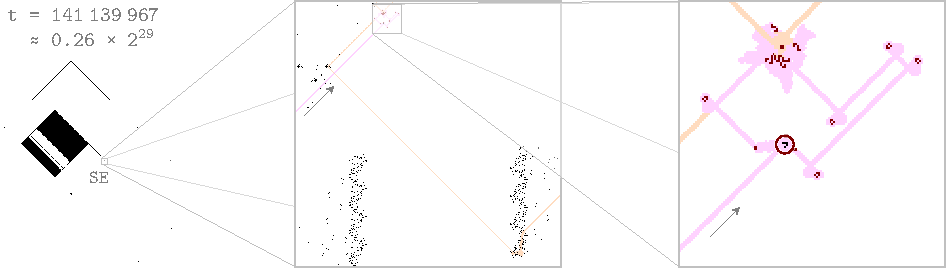
\includegraphics[width=1\textwidth]{0e0p/0e0p_timeline_141139967.pdf}}
	\caption{The southeast child's shell has been constructed. A single stray glider (circled in \bgbox{redback}{red}) is about to delete a Snark, allowing the rest of the construction recipe to enter the correct lane of the child's shell. This ensures that the rest of that child is constructed in the proper orientation.}
	\label{fig:0e0p_timeline_141139967}
\end{figure}

The kernel takes a bit more than twice as long to construct as the shell, and makes use of numerous long-distance Cordership-based elbow pushes. This construction is heavily unoptimized, as it was generated automatically by slsparse using known standard methods---fire a Cordership towards a location, build something there, fire a glider back, and repeat.

However, this could be made much less expensive. For example, instead of using a long-distance Cordership-based elbow push to start construction of the \texttt{CN} construction site (which is done at $t = 181{\thousep}162{\thousep}958 \approx 0.3374 \times 2^{29}$), it would have been possible to aim gliders at an outlying still life in the unused circuitry near the construction point along the northwest edge, produce a new target object, then rebuild the temporarily sacrificed still life. The 0E0P metacell could be reduced in size and made to run several times faster with these kinds of optimizations---but it would have been far more difficult to complete a working pattern.

The last part of the kernel to be constructed is its south corner, which begins at generation $t = 367{\thousep}748{\thousep}078 \approx 0.6850 \times 2^{29}$ (see Figure~\ref{fig:0e0p_timeline_367748078}). The entirety of the metacell's clock gun and logic circuitry has been constructed at this point. The final glider used in the south corner's construction is emitted at $t = 430{\thousep}473{\thousep}285 \approx 0.8018 \times 2^{29}$, followed by a Snarkmaker recipe that is used to redirect the rest of the single-channel glider recipe towards the nucleus.

\begin{figure}[!htb]
	\centering
	\embedlink{0e0p_timeline_367748078_small}{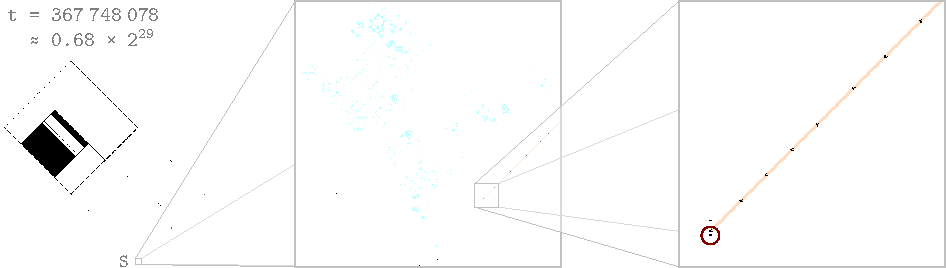
\includegraphics[width=1\textwidth]{0e0p/0e0p_timeline_367748078.pdf}}
	\caption{Construction of the child's south corner begins. The logic circuit (highlighted in \bgbox{aquaback}{aqua}, including the clock gun) will now be constructed by the elbow block circled in \bgbox{redback}{red}.}
	\label{fig:0e0p_timeline_367748078}
\end{figure}


%%%%%%%%%%%%%%%%%%%%%%
\subsection{Generations $\mathbf{0.80 \times 2^{29}}$ to $\mathbf{0.82 \times 2^{29}}$: CN and CE Loop Initialization}\label{sec:0e0p_timeline_nucleus_nw}
%%%%%%%%%%%%%%%%%%%%%%

A single ``trigger'' glider passes through the Snark that was just created at the south end of the kernel, and is redirected towards a temporary Snark that it passes through at generation $t = 431{\thousep}312{\thousep}741 \approx 0.8034 \times 2^{29}$ (see Figure~\ref{fig:0e0p_timeline_431312741}). That glider then travels northeast and then northwest so as to initialize the \texttt{CN} subroutine loop. The single-channel glider recipe that will fill that loop will follow the same path shortly afterwards.

\begin{figure}[!htb]
	\centering
	\embedlink{0e0p_timeline_431312741_small}{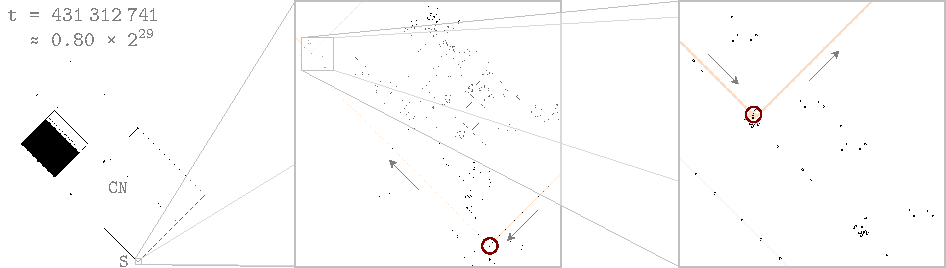
\includegraphics[width=1\textwidth]{0e0p/0e0p_timeline_431312741.pdf}}
	\caption{The child's kernel has been constructed. A glider goes through the final Snark that was constructed at the south corner of its kernel (circled in \bgbox{redback}{red} in the middle) and then is redirected through another temporary Snark (circled in \bgbox{redback}{red} on the right) that leads it to \texttt{CN}, which will trigger construction of the nucleus's northwest wall.}
	\label{fig:0e0p_timeline_431312741}
\end{figure}

By $t = 431{\thousep}969{\thousep}616 \approx 0.8046 \times 2^{29}$, the leading trigger glider reaches a temporary Snark in the \texttt{CN} subroutine storage loop (see Figure~\ref{fig:0e0p_timeline_431969616}). It then goes through a splitter at $t = 431{\thousep}969{\thousep}830$ and initializes the period $2^{29}$~clock gun there at $t = 431{\thousep}971{\thousep}416$, which will destroy the period $2^{21}$ storage loop after it has been used $2^{29}/2^{21} = 256$ times.

\begin{figure}[!htb]
	\centering
	\embedlink{0e0p_timeline_431969616_small}{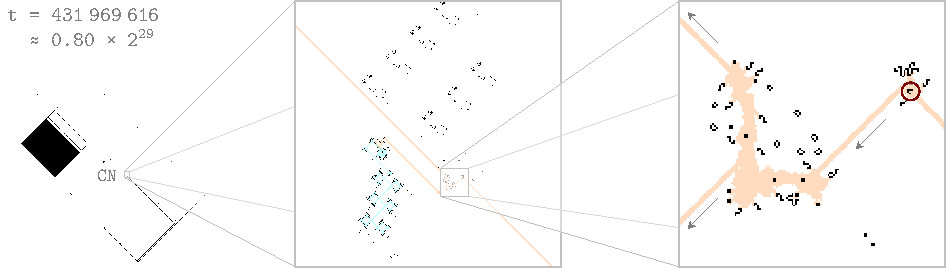
\includegraphics[width=1\textwidth]{0e0p/0e0p_timeline_431969616.pdf}}
	\caption{The glider from Figure~\ref{fig:0e0p_timeline_431312741} (circled in \bgbox{redback}{red}) has reached \texttt{CN} and is about to start the clock there (highlighted in \bgbox{aquaback}{aqua}). That clock will trigger \texttt{CN}'s self-destruction $2^{29}$ generations later, after the period $2^{21}$ \texttt{CN} subroutine loop has been used $2^8 = 256$ times.}
	\label{fig:0e0p_timeline_431969616}
\end{figure}

The single-channel recipe following the trigger glider then goes through the same splitter, to be duplicated several times into four streams heading southwest that construct the northwest wall of the nucleus, and also to be copied into the storage loop where it will eventually re-enter this same splitter again, 255 more times. The final glider in that portion of the single-channel recipe enters the loop at $t = 433{\thousep}582{\thousep}348 \approx 0.8076 \times 2^{29}$ (see Figure~\ref{fig:0e0p_timeline_433582348}).

\begin{figure}[!htb]
	\centering
	\embedlink{0e0p_timeline_433582348_small}{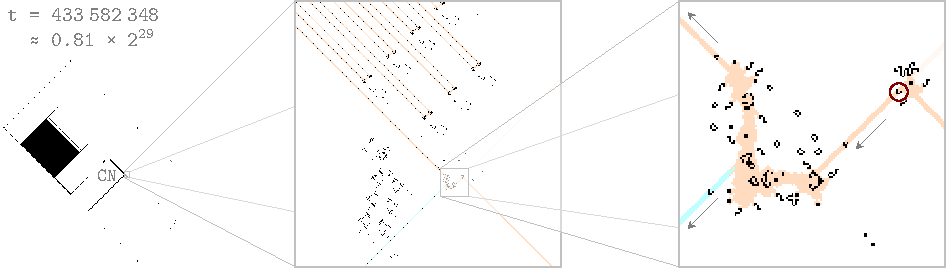
\includegraphics[width=1\textwidth]{0e0p/0e0p_timeline_433582348.pdf}}
	\caption{The subroutine glider loop at \texttt{CN} is now filled, since its final glider (circled in \bgbox{redback}{red}) just passed through the same temporary Snark as in Figure~\ref{fig:0e0p_timeline_431969616}, which will soon be destroyed by the glider from Figures~\ref{fig:0e0p_timeline_431312741} and \ref{fig:0e0p_timeline_431969616}. The gliders leaving from the \bgbox{aquaback}{aqua} lane of the splitter are duplicated three more times and then head to \texttt{LW} to construct the northwest wall of the nucleus.}
	\label{fig:0e0p_timeline_433582348}
\end{figure}

That loop of gliders can be seen having constructed the first set of $8$ Snarks along the northwest wall of the nucleus by generation $t = 434{\thousep}341{\thousep}913 \approx 0.8090 \times 2^{29}$ in Figure~\ref{fig:0e0p_timeline_434341913}. This $8$-Snark construction is repeated a total of $256$ times along this northwest wall (for a total $1{\thousep}024$ reflectors made up of $2$ Snarks each).

\begin{figure}[!htb]
	\centering
	\embedlink{0e0p_timeline_434341913_small}{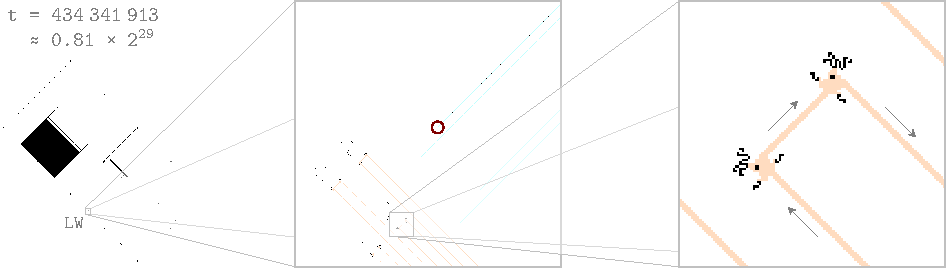
\includegraphics[width=1\textwidth]{0e0p/0e0p_timeline_434341913.pdf}}
	\caption{The subroutine glider loop has been used once at \texttt{LW} to construct the first set of Snarks along the nucleus's northwest wall (the last elbow operation from that loop is about to pull the elbow block circled in \bgbox{redback}{red} by 14fd). The glider from Figure~\ref{fig:0e0p_timeline_431312741} is between \texttt{CE} and \texttt{SE}, on its way to \texttt{S}.}
	\label{fig:0e0p_timeline_434341913}
\end{figure}

After the subroutine storage loop is filled back in Figure~\ref{fig:0e0p_timeline_433582348}, the input Snark from that figure must be removed because it's directly in the way of the circulating recipe in the storage loop. The trigger glider does this, and the Snark is completely erased as of $t = 434{\thousep}725{\thousep}275 \approx 0.8097 \times 2^{29}$. The trigger glider then travels southeast, and then southwest, back to the child metacell's south corner, where it will destroy and be destroyed by the Snark from Figure~\ref{fig:0e0p_timeline_431312741} that sent it to the \texttt{CN} storage loop in the first place. This final act of the trigger glider takes place at $t = 434{\thousep}724{\thousep}270 \approx 0.8097 \times 2^{29}$ (see Figure~\ref{fig:0e0p_timeline_434724270}).

\begin{figure}[!htb]
	\centering
	\embedlink{0e0p_timeline_434724270_small}{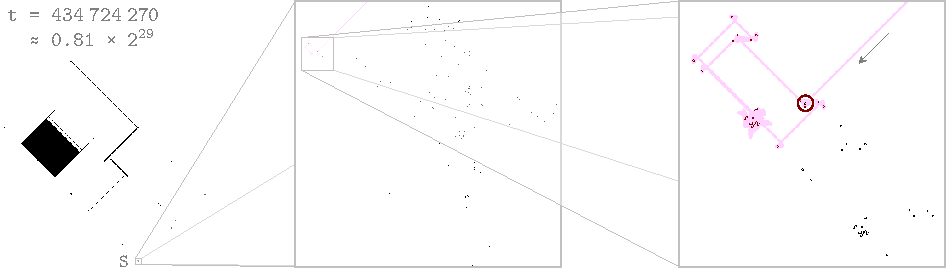
\includegraphics[width=1\textwidth]{0e0p/0e0p_timeline_434724270.pdf}}
	\caption{The glider from Figure~\ref{fig:0e0p_timeline_431312741} makes it back to \texttt{S}, where it destroys (and is destroyed by) the Snark from that figure. This opens a path toward the \texttt{CE} construction location, which will be used soon.}
	\label{fig:0e0p_timeline_434724270}
\end{figure}

The entire procedure used to initialize the \texttt{CN} subroutine loop, as described by Figures~\ref{fig:0e0p_timeline_431312741}--\ref{fig:0e0p_timeline_434724270}, then repeats for the \texttt{CE} subroutine loop. At $t = 435{\thousep}925{\thousep}955 \approx 0.8120 \times 2^{29}$, the trigger glider for the \texttt{CE} subroutine recipe passes through the location where the Snark from Figure~\ref{fig:0e0p_timeline_434724270} used to be, and instead goes into a Snark that directs it to \texttt{CE} (see Figure~\ref{fig:0e0p_timeline_435925955}).

\begin{figure}[!htb]
	\centering
	\embedlink{0e0p_timeline_435925955_small}{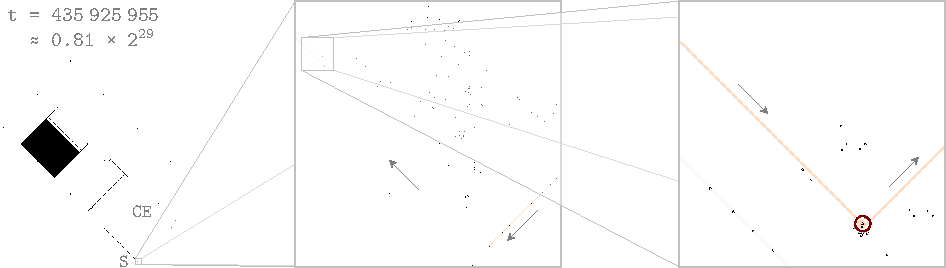
\includegraphics[width=1\textwidth]{0e0p/0e0p_timeline_435925955.pdf}}
	\caption{A glider goes through a Snark at the child's south corner that leads it to \texttt{CE}, which will trigger construction of the nucleus's southeast wall (just like the glider from Figure~\ref{fig:0e0p_timeline_431312741}). The same things as in Figures~\ref{fig:0e0p_timeline_431969616}--\ref{fig:0e0p_timeline_434341913} then happen, but along that southeast wall instead of the northwest one.}
	\label{fig:0e0p_timeline_435925955}
\end{figure}

That trigger glider will then activate the clock gun located at \texttt{CE} at $t = 436{\thousep}382{\thousep}282 \approx 0.8128 \times 2^{29}$, in the exact same way as happened at \texttt{CN} in Figure~\ref{fig:0e0p_timeline_431969616}. The subroutine portion of the single-channel recipe then fills the loop, with its final glider entering the loop at $t = 437{\thousep}805{\thousep}347 \approx 0.8155 \times 2^{29}$. Once this glider passes through this temporary Snark, the full construction recipe of the 0E0P metacell has been completely processed.

The trigger glider then destroys the \texttt{CE} subroutine loop's input Snark, and is then redirected along a self-destruct chain toward the child's south corner, removing reflectors in four more locations along the way. Finally, it destroys (and is destroyed by) the Snark that directed it to \texttt{CE} in the first place. This final usage of the trigger glider occurs at $t = 438{\thousep}935{\thousep}522 \approx 0.8176 \times 2^{29}$ (see Figure~\ref{fig:0e0p_timeline_438935522}).

\begin{figure}[!htb]
	\centering
	\embedlink{0e0p_timeline_438935522_small}{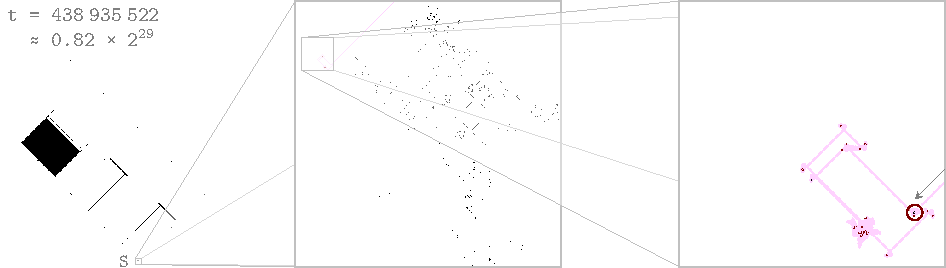
\includegraphics[width=1\textwidth]{0e0p/0e0p_timeline_438935522.pdf}}
	\caption{The glider from Figure~\ref{fig:0e0p_timeline_435925955} makes it back to \texttt{S}, where it destroys (and is destroyed by) the Snark from that figure. A complete copy of the construction recipe from the parent metacell has now been used---the next copy will be directed into the nucleus of this child.}
	\label{fig:0e0p_timeline_438935522}
\end{figure}

Thanks to the removal of this Snark, the \emph{next} copy of the single-channel glider recipe that comes into this child metacell will be fed into the Snarks that make up the nucleus's walls, rather than to the \texttt{CN} or \texttt{CE} subroutine loops. Those nucleus walls are still being constructed by the subroutine loops, which won't complete for roughly $2^{29}$ more generations, but the nucleus construction process moves at roughly the same speed as the approaching recipe, so the construction will safely complete before the recipe gets there.


%%%%%%%%%%%%%%%%%%%%%%
\subsection{Generations $\mathbf{0.82 \times 2^{29}}$ to $\mathbf{2 \times 2^{29}}$: Activation of the Southeast Child}\label{sec:0e0p_timeline_nucleus_fill}
%%%%%%%%%%%%%%%%%%%%%%

Now both subroutine loops of the child metacell are filled and are building the repetitive Snark chains that will hold its copy of the single-channel glider recipe. When construction is done there will be 256 copies of 8 Snarks in long chains along the northwest and southeast walls of the nucleus. The sets of 8 Snarks and their associated self-destruct circuitry are not quite mirror images of each other, so different recipes are needed in the \texttt{CN} and \texttt{CE} subroutine loops.

This construction and filling of the nucleus goes on for quite a while. The subroutine storage loops are period $2^{21}$, and they have to cycle $256$ times each before being shut down by the period $256 \times 2^{21} = 2^{29}$ clock guns. Splitters near the storage units duplicate the recipe several times, so that construction actually proceeds on four Snark pairs simultaneously. The unit of repetition that's constructed $256$ times is made up of eight gliders, offset in pairs from each other so that the simultaneous constructions don't get in each other's way.

At generation $t = 968{\thousep}843{\thousep}520 \approx 1.8046 \times 2^{29}$, the northwest wall of Snarks is complete, and a Herschel is present in the \texttt{CN} subroutine clock's gun that will produce the glider that makes it through all of the twenty-one semi-Snarks in the loops below (see Figure~\ref{fig:0e0p_timeline_968843520}). That signal destroys a block in a syringe in that subroutine loop, so that all further recipe gliders in the loop will be harmlessly absorbed by the syringe's eater~2---no more building will occur.

\begin{figure}[!htb]
	\centering
	\patternlink{0e0p_timeline_968843520_small}{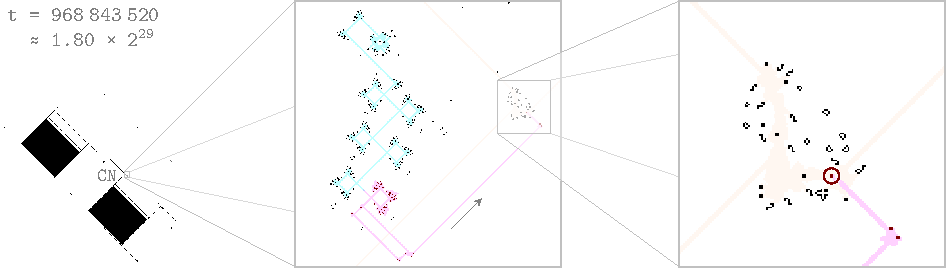
\includegraphics[width=1\textwidth]{0e0p/0e0p_timeline_968843520.pdf}}
	\caption{A Herschel is present in the \texttt{CN} clock gun that will produce the glider that makes it through all of the twenty-one semi-Snarks in the loops below. That signal destroys a block in a syringe (circled in \bgbox{redback}{red}), so that the \texttt{CN} storage loop stops building the northwest wall of the nucleus. This same glider also destroys the three outermost semi-Snarks, making the clock gun $8$ times faster.}
	\label{fig:0e0p_timeline_968843520}
\end{figure}

A side branch of that same signal also starts the gradual process of dismantling the subroutine clock gun. This first output glider destroys three of the clock gun's semi-Snarks, making it 8 times faster, and every subsequent output glider acts similarly. The result of this is that the clock gun did nothing for a long time ($2^{29}$ generations), and then its destruction happens faster and faster.

For example, the \emph{next} three semi-Snarks are destroyed just $2^{26}$ generations later, by the Herschel that appears at $t = 1{\thousep}035{\thousep}952{\thousep}384 \approx 1.9296 \times 2^{29}$, and the clock gun vanishes completely just a bit more than $2^{24}$ generations after that, at $t = 1{\thousep}054{\thousep}065{\thousep}485 \approx 1.9633 \times 2^{29}$. The entirety of the \texttt{CN} storage loop is similarly gone just a few thousand generations later, at $t = 1{\thousep}054{\thousep}073{\thousep}568$. The \texttt{CE} subroutine clock and storage loop self-destruct in the exact same way shortly thereafter, and are gone as of $t = 1{\thousep}058{\thousep}486{\thousep}020 \approx 1.9716 \times 2^{29}$.

Back in time slightly at $t = 974{\thousep}368{\thousep}517 \approx 1.8149 \times 2^{29}$, after construction of the Snark walls finished but before the subroutine storage loops self-destructed, the final glider in the single-channel recipe is about to enter the child's nucleus at \texttt{INS} (see Figure~\ref{fig:0e0p_timeline_974368517}). Once this insertion is complete, the child's nucleus will be fully populated with a copy of the parent's DNA.

\begin{figure}[!htb]
	\centering
	\patternlink{0e0p_timeline_974368517_small}{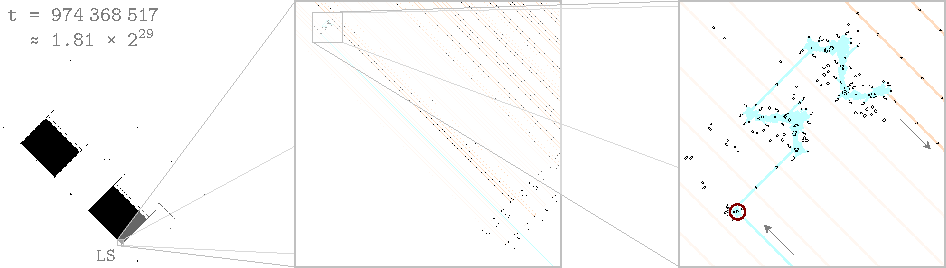
\includegraphics[width=1\textwidth]{0e0p/0e0p_timeline_974368517.pdf}}
	\caption{The final glider in the 0E0P's single-channel glider recipe is injected into the child's nucleus, at the location circled in \bgbox{redback}{red}.}
	\label{fig:0e0p_timeline_974368517}
\end{figure}

After the first glider in the child's nucleus makes it all the way through the long back-and-forth Snark chains for the first time, it arrives at a splitter at the south corner at $t = 1{\thousep}073{\thousep}734{\thousep}584 \approx 2.0000 \times 2^{29}$. It then uses one-time circuitry to start up the child's clock gun (see Figure~\ref{fig:0e0p_timeline_1073734584}), aligned exactly with the timing of the parent's clock gun. However, the clock gun does not actually do anything until much later, when an eater is removed from its path.

\begin{figure}[!htb]
	\centering
	\patternlink{0e0p_timeline_1073734584_small}{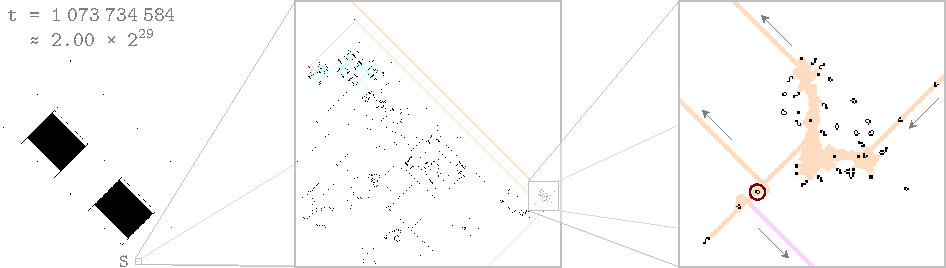
\includegraphics[width=1\textwidth]{0e0p/0e0p_timeline_1073734584.pdf}}
	\caption{The first gliders in the child's single-channel glider recipe complete their first journey through its nucleus. The very first of these gliders hits a one-time reflector (circled in \bgbox{redback}{red}) that redirects it to start up that child metacell's clock gun (highlighted in \bgbox{aquaback}{aqua}).}
	\label{fig:0e0p_timeline_1073734584}
\end{figure}

At this point, the southeast child is fully constructed and simply waits until the parent metacell's other neighbors are constructed before really doing anything. The single-channel glider recipe will cycle through its nucleus several times before it is actually made to do anything of note.


%%%%%%%%%%%%%%%%%%%%%%
\subsection{Generations $\mathbf{2 \times 2^{29}}$ to $\mathbf{8 \times 2^{29}}$: Construction of the Other Children}\label{sec:0e0p_timeline_other_child}
%%%%%%%%%%%%%%%%%%%%%%

Back in the parent metacell, at $t = 1{\thousep}073{\thousep}741{\thousep}824 = 2 \times 2^{29}$, a Herschel is present in the south clock gun. This Herschel will produce a glider that removes an eater~1 blocking the period~$2^{25}$ branch of the clock gun (see Figure~\ref{fig:0e0p_timeline_1073741824}). Exactly $2^{25}$ generations later, at $t = 1{\thousep}107{\thousep}296{\thousep}256$, a Herschel in the same location uses one-time circuitry to switch over to building the northeast child metacell.

\begin{figure}[!htb]
	\centering
	\embedlink{0e0p_timeline_1073741824_small}{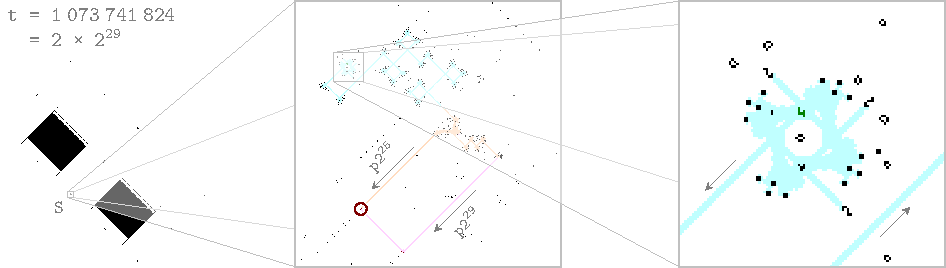
\includegraphics[width=1\textwidth]{0e0p/0e0p_timeline_1073741824.pdf}}
	\caption{A Herschel is present in the south clock gun of the parent metacell (highlighted in \bgbox{aquaback}{aqua}), which releases a glider that uses a one-time turner to destroy an eater~1 (circled in \bgbox{redback}{red}), thus initiating construction of the northeast child.}
	\label{fig:0e0p_timeline_1073741824}
\end{figure}

At $t = 1{\thousep}610{\thousep}612{\thousep}736 = 3 \times 2^{29}$, the next ``$2^{29}$'' Herschel appears in the clock gun. However, despite the resulting glider making it past all $21$ semi-Snarks in the clock gun, it does not actually do anything of note---there is a block along the period $2^{29}$ output lane that simply absorbs it. This block causes another $2^{29}$-generation cycle to occur, so that the single-channel glider recipe is sent to the northeast child metacell twice: once to do the construction, and once to populate the new child's nucleus with a copy of the recipe. Blocks along the clock gun's output lane are similarly used to absorb the output gliders that are produced by Hershels at $t = 2^{29}$, $t = 5 \times 2^{29}$, and $t = 7 \times 2^{29}$.

By generation $t = 2{\thousep}147{\thousep}483{\thousep}648 = 4 \times 2^{29}$, the northeast child's nucleus has been filled and its clock gun has started up. A Herschel is present in the south clock gun that will produce a glider that removes an eater~1 from the period $2^{25}$ output lane of the clock gun, and then exactly $2^{25}$ generations later (at $t = 2{\thousep}181{\thousep}038{\thousep}080$) another Herschel is present in the clock gun that will use one-time circuitry to switch over to construction of the northwest child metacell (see Figure~\ref{fig:0e0p_timeline_2147483648}).

\begin{figure}[!htb]
	\centering
	\embedlink{0e0p_timeline_2147483648_small}{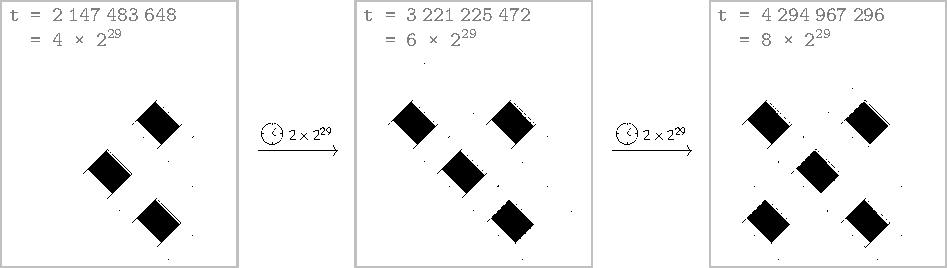
\includegraphics[width=1\textwidth]{0e0p/0e0p_timeline_2147483648.pdf}}
	\caption{The parent metacell constructs its children in the following order: southeast, northeast, northwest, southwest. It takes $2 \times 2^{29}$ generations to build a single child and populate its nucleus.}
	\label{fig:0e0p_timeline_2147483648}
\end{figure}

By generation $t = 3{\thousep}221{\thousep}225{\thousep}472 = 6 \times 2^{29}$, the northwest child has been constructed and had its nucleus filled, and another Herschel is present in the clock gun lead to the parent metacell starting construction of the southwest child. Finally, all four child metacells have been constructed and had their nuclei filled by $t = 4{\thousep}294{\thousep}967{\thousep}296 = 8 \times 2^{29}$.


%%%%%%%%%%%%%%%%%%%%%%
\subsection{Generations $\mathbf{8 \times 2^{29}}$ to $\mathbf{14 \times 2^{29}}$: Preliminary Clean-Up}\label{sec:0e0p_timeline_prelim_cleanup}
%%%%%%%%%%%%%%%%%%%%%%

Nothing of importance happens in either the parent or child metacells between generations $8 \times 2^{29}$ and $12 \times 2^{29}$---they both just loop the single-channel recipe through their nuclei a few times. In the parent metacell, the output of the south clock gun hits a sequence of four blocks along the period~$2^{29}$ output lane (which can be seen near the southwest end of that lane in Figure~\ref{fig:0e0p_clock_gun_full}), simply causing it to do nothing for these generations. In the child metacells, the output of the south clock gun is still being absorbed by an eater~1 (which is circled in red at the northeast end of the output lane in Figure~\ref{fig:0e0p_clock_gun_full}).

At $t = 6{\thousep}442{\thousep}450{\thousep}944 = 12 \times 2^{29}$, the parent metacell's south clock gun is holding a Herschel that will release a glider, which destroys a single Snark elsewhere at its south corner. This Snark was used by the metacell when it was a child, after computing its state, to store that state in a sequence of up to 8 blocks.\footnote{This Snark is destroyed now, instead of during the ``main'' self-destruction stage at $t = 15 \times 2^{29}$, just as a minor convenience---the 0E0P metacell could be rewired to destroy it later instead.}

More interesting things finally start happening $2^{29}$ generations later: at $t = 6{\thousep}979{\thousep}321{\thousep}856 = 13 \times 2^{29}$, a Herschel is present in the parent's south clock gun that will release a glider, which will use one-time circuitry to destroy a block from a syringe in the part of the nucleus memory loop that extends through the metacell's south corner (see Figure~\ref{fig:0e0p_timeline_6979321856}). On the next cycle of the single-channel glider recipe through the nucleus, all gliders will be absorbed by that syringe's eater~2, so the recipe will gradually empty out of the nucleus over the course of those $2^{29}$ generations, with the final glider being absorbed at $t = 7{\thousep}516{\thousep}189{\thousep}238 \approx 14.0000 \times 2^{29}$.

\begin{figure}[!htb]
	\centering
	\embedlink{0e0p_timeline_6979321856_small}{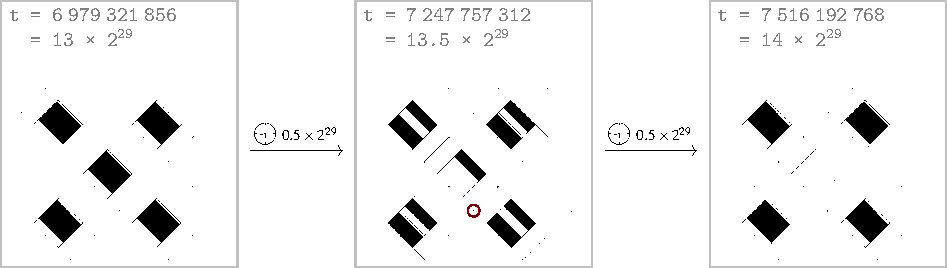
\includegraphics[width=1\textwidth]{0e0p/0e0p_timeline_6979321856.pdf}}
	\caption{A Herschel is present in the parent metacell's control clock gun that is used to erase a block from a syringe, so that the contents of its nucleus are absorbed over the next $2^{29}$ generations (at the location circled in \bgbox{redback}{red}).}
	\label{fig:0e0p_timeline_6979321856}
\end{figure}

% Exercise idea: At approximately what generation will (piece) of the (northwest) child be constructed? Can be figured out by combining various stages in this timeline


%%%%%%%%%%%%%%%%%%%%%%
\subsection{Generations $\mathbf{14 \times 2^{29}}$ to $\mathbf{15 \times 2^{29}}$: State Information is Sent to Children}\label{sec:0e0p_timeline_state}
%%%%%%%%%%%%%%%%%%%%%%

After their nuclei are empty, parent metacells send their state to their children, so that those children will be able to compute their own states. This process is initiated at $t = 7{\thousep}516{\thousep}192{\thousep}768 = 14 \times 2^{29}$, when a Herschel is present in the parent metacell's clock gun that will fire $8$ gliders at the $0$--$6$ or $8$ blocks that store its state. As a result, $0$ or $2$--$8$ gliders will escape (representing the metacell's state $0$ or $1$--$7$),\footnote{In the example that we are illustrating, the parent metacell is in state $7$, so there are $0$ blocks, and all $8$ gliders will escape.} as illustrated in Figure~\ref{fig:0e0p_timeline_7516192768}.

\begin{figure}[!htb]
	\centering
	\embedlink{0e0p_timeline_7516192768_small}{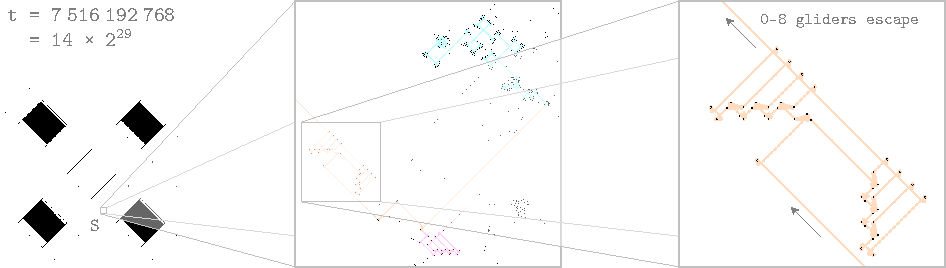
\includegraphics[width=1\textwidth]{0e0p/0e0p_timeline_7516192768.pdf}}
	\caption{A Herschel is present in the south clock gun of the parent metacell (highlighted in \bgbox{aquaback}{aqua}), which releases a glider that uses one-time circuitry to send its state (which is currently stored in a sequence of $0$--$8$ blocks) to its children (as a sequence of $0$--$8$ gliders). Some mild cleanup also happens at this stage---the four state-reading boats (if any of them still exist, highlighted in \bgbox{magentaback}{magenta}) from the upcoming Figure~\ref{fig:0e0p_timeline_7517755585} are destroyed.}
	\label{fig:0e0p_timeline_7516192768}
\end{figure}

Those gliders follow a spiral path through the kernel into the south ``\texttt{logic}'' area of each of the children (regardless of whether or not this particular parent metacell built that child). When the state gliders arrive at a child's ``\texttt{logic}'' area, the first glider (if it exists) hits one-time circuitry that erases the eater~1 blocking the clock gun's p$2^{29}$ output lane, while the remaining $0$--$7$ gliders are used to destroy $0$--$7$ blocks in the logic circuitry, thus storing the parent's state in the child. The state gliders arrive at the four child metacells at slightly different times, in the following order:\smallskip

\begin{itemize}
	\item \textbf{SW child}: at $t = 7{\thousep}517{\thousep}755{\thousep}585 \approx 14.0029 \times 2^{29}$ (see Figure~\ref{fig:0e0p_timeline_7517755585}).\smallskip
	
	\item \textbf{NE child}: just $2{\thousep}052$ generations later, at $t = 7{\thousep}517{\thousep}757{\thousep}637$.\smallskip
	
	\item \textbf{NW child}: at $t = 7{\thousep}518{\thousep}791{\thousep}855 \approx 14.0048 \times 2^{29}$.\smallskip
	
	\item \textbf{SE child}: just $2{\thousep}892$ generations later, at $t = 7{\thousep}518{\thousep}794{\thousep}747$.\smallskip
\end{itemize}

\begin{figure}[!htb]
	\centering
	\embedlink{0e0p_timeline_7517755585_small}{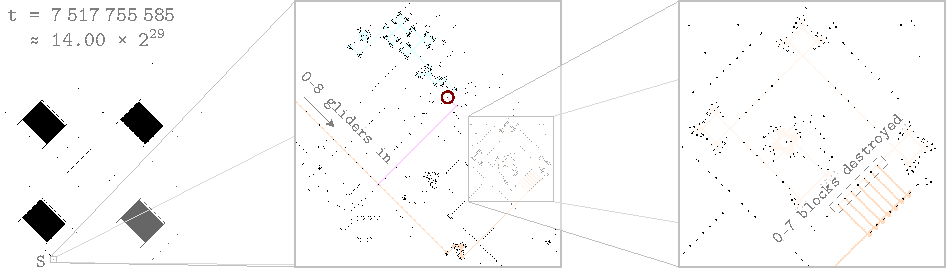
\includegraphics[width=1\textwidth]{0e0p/0e0p_timeline_7517755585.pdf}}
	\caption{State gliders from parent metacells arrive at their southwest children. The first of these gliders hits a one-time turner (a boat, mentioned in the caption of Figure~\ref{fig:0e0p_timeline_7516192768}) and then destroys the eater~1 blocking the period~$2^{29}$ output lane of that child's south clock gun (circled in \bgbox{redback}{red}). The other $0$--$7$ state gliders destroy $0$--$7$ blocks along the path of the state-lookup clock gun (here, the parent metacell was in state $7$, so $7$ gliders destroy $7$ blocks).}
	\label{fig:0e0p_timeline_7517755585}
\end{figure}

Since every child metacell has a parent, a non-zero state will be sent in from at least one the four possible directions, so the eater~1 blocking the south clock gun's period~$2^{29}$ output lane will always be destroyed. Also, state information arrives from the (up to) four parents on slightly different lanes, so that state gliders from different parents destroy different blocks in the state-lookup clock gun.


%%%%%%%%%%%%%%%%%%%%%%
\subsection{Generations $\mathbf{15 \times 2^{29}}$ to $\mathbf{16 \times 2^{29}}$: Child State Computation and Parent Self-Destruction}\label{sec:0e0p_timeline_self_dest}
%%%%%%%%%%%%%%%%%%%%%%

Now that child metacells have recorded the states of their parents (in the absence of certain blocks in their state-lookup clock guns), it is time for them to compute their own states. To do this, a Herschel is present in each child's south clock gun at $t = 8{\thousep}053{\thousep}063{\thousep}680 = 15 \times 2^{29}$ that triggers its state-lookup clock gun to start.\index{state-lookup clock gun} That state-lookup gun will be ready to compute the metacell's state $8{\thousep}846$ generations later, at $t = 8{\thousep}053{\thousep}072{\thousep}526$ (see Figure~\ref{fig:0e0p_timeline_8053072526}).

\begin{figure}[!htb]
	\centering
	\embedlink{0e0p_timeline_8053072526_small}{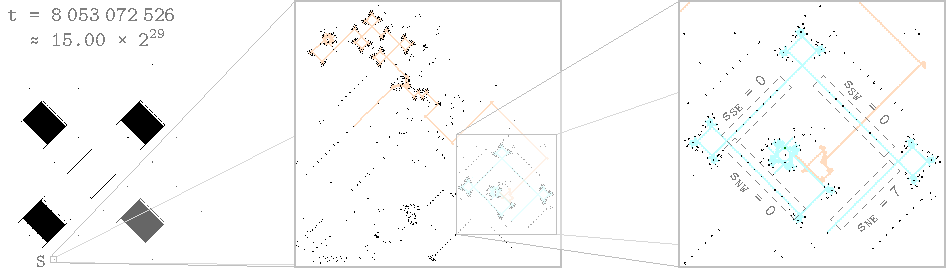
\includegraphics[width=1\textwidth]{0e0p/0e0p_timeline_8053072526.pdf}}
	\caption{The state-lookup clock gun (highlighted in \bgbox{aquaback}{aqua}) has been started in the child metacells. In the southwest child metacell (magnified here), the parent metacell to the northeast had state $7$, which is encoded in the fact that $7$ blocks are missing along one of the clock gun's edges. The leftover arrangement of blocks make it so that the central period $1{\thousep}024$ gun releases $(7-s_{\textup{NW}}) + 8(7-s_{\textup{SE}}) + 64(7-s_{\textup{SW}}) + 512(7-s_{\textup{NE}}) = 511$ gliders before one escapes.}
	\label{fig:0e0p_timeline_8053072526}
\end{figure}

This period~$1{\thousep}024$ state-lookup gun works as described in Section~\ref{sec:0e0p_structure_logic}: if we label the states of the northwest, southeast, southwest, and northeast parents by $s_{\textup{NW}}$, $s_{\textup{SE}}$, $s_{\textup{SW}}$, and $s_{\textup{NE}}$, respectively, then
\[
	(7-s_{\textup{NW}}) + 8(7-s_{\textup{SE}}) + 64(7-s_{\textup{SW}}) + 512(7-s_{\textup{NE}})
\]
gliders are absorbed by blocks and semi-Snarks before any escape.\footnote{In the notation of Section~\ref{sec:0e0p_structure_logic}, we have $a = 7-s_{\textup{NW}}$, $b = 7-s_{\textup{SE}}$, $c = 7-s_{\textup{SW}}$, and $d = 7-s_{\textup{NE}}$. This particular ordering of which neighbors corresponds to ``$a$'', ``$b$'', ``$c$'', and ``$d$'' is unimportant---it's just a result of how it was easiest to wire the 0E0P.} That first escaping glider is thus generated by the Herschel that is present in it at generation
\begin{align*}
	t & = 15 \times 2^{29} + 8846 + 1024\big((7-s_{\textup{NW}}) + 8(7-s_{\textup{SE}}) + 64(7-s_{\textup{SW}}) + 512(7-s_{\textup{NE}})\big).
\end{align*}

For example, consider the southwest child of the metacell that we have been tracking. It has a northeast parent in state $7$, and all other parents in state $0$ (since they do not exist), so the first glider to make it out of its state-lookup gun does so via the Herschel that is present at generation
\begin{align*}
	t & = 15 \times 2^{29} + 8846 + 1024\big((7-0) + 8(7-0) + 64(7-0) + 512(7-7)\big) \\
	& = 8{\thousep}053{\thousep}595{\thousep}790 \approx 15.0010 \times 2^{29}.
\end{align*}
That glider escaping the state-lookup gun causes it to self-destruct and then emit a pair of gliders: one that destroys an eater at $t = 8054286989 \approx 15.0023 \times 2^{29}$, unblocking the single-channel glider stream,\footnote{This timestamp is specific to the southwest child. Children with different parent state configurations will have this happen slightly earlier or later.} and one that destroys a block in a syringe just $972$ generations later, re-blocking the stream. The result is that an approximately $900$-generation chunk of the 0E0P's rule table is copied---a portion containing $0$--$7$ gliders that describe the new state of this child metacell (see Figure~\ref{fig:0e0p_timeline_8054286989}).

\begin{figure}[!htb]
	\centering
	\embedlink{0e0p_timeline_8054286989_small}{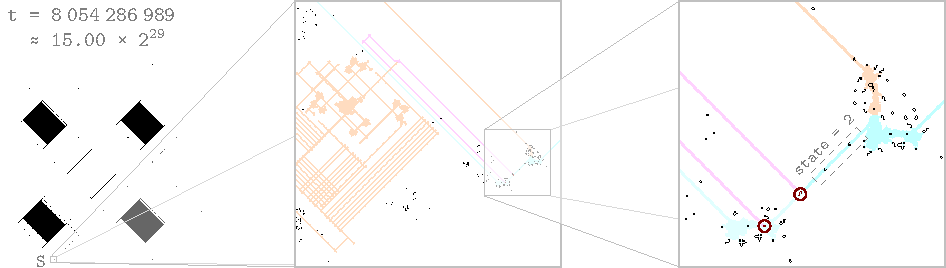
\includegraphics[width=1\textwidth]{0e0p/0e0p_timeline_8054286989.pdf}}
	\caption{The southwest child's state ($2$) being extracted from the lookup table. A glider destroys an eater~1 (at the top-right location circled in \bgbox{redback}{red}), unblocking a portion of the lookup table, and another glider destroys a block (at the bottom-left location circled in \bgbox{redback}{red}), re-blocking it $972$ generations later.}
	\label{fig:0e0p_timeline_8054286989}
\end{figure}

The state-lookup gun of this southwest child thus extracts the $512$th chunk of the lookup table, which contains $2$ gliders, indicating that its state is $2$. The other three children look at different chunks of the lookup table and thus extract different states:\smallskip

\begin{itemize}
	\item \textbf{NE child}: The state-lookup clock gun extracts the
	\[
		1 + (7-0) + 8(7-0) + 64(7-7) + 512(7-0) = 3{\thousep}648\text{th}
	\]
	chunk of the lookup table, which contains $4$ gliders, so its state is $4$.\smallskip
	
	\item \textbf{NW child}: Extracts the $1 + (7-0) + 8(7-7) + 64(7-0) + 512(7-0) = 4{\thousep}040\text{th}$ chunk of the lookup table, which contains $1$ glider, so its state is $1$.\smallskip
	
	\item \textbf{SE child}: Extracts the $1 + (7-7) + 8(7-0) + 64(7-0) + 512(7-0) = 4{\thousep}089\text{th}$ chunk of the lookup table, which contains $6$ gliders, so its state is $6$.\smallskip
\end{itemize}

After the children's states are extracted in the form of $0$--$7$ gliders, the first glider (if it exists) is duplicated, resulting in a sequence of $0$ or $2$--$8$ gliders, and erases some one-time circuitry that would otherwise cause the metacell to die early. The resulting sequence of gliders is then redirected toward a sequence of $8$ blocks, so that the state can be stored for a long period of time in their absences. In the southwest child, this happens at $t = 8{\thousep}054{\thousep}294{\thousep}330$ (see Figure~\ref{fig:0e0p_timeline_8054294330}).

\begin{figure}[!htb]
	\centering
	\embedlink{0e0p_timeline_8054294330_small}{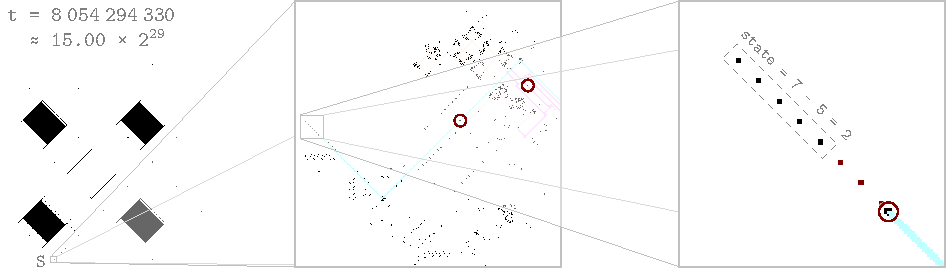
\includegraphics[width=1\textwidth]{0e0p/0e0p_timeline_8054294330.pdf}}
	\caption{The southwest child's $2$ state gliders erasing one-time circuitry that would otherwise cause the metacell to die early (highlighted in \bgbox{magentaback}{magenta}), and storing their state in the $8$-block sequence at the west edge of the south corner. The first of those $2$ state gliders was duplicated, so $3$ gliders (circled in \bgbox{redback}{red}) will hit the blocks, leaving $8-3 = 5$ blocks behind, corresponding to a the child's state $7 - 5 = 2$.}
	\label{fig:0e0p_timeline_8054294330}
\end{figure}

% Exercise: what generation does glider escape in some other configuration or for some other child? e.g., what generation does northeast child extract its state? When are those state gliders stored in the blocks?

Meanwhile, parent metacells have served their purpose, so they are free to die. The Herschels that are present in \emph{their} south clock guns at generation $t = 8{\thousep}053{\thousep}063{\thousep}680 = 15 \times 2^{29}$ trigger this self-destruction. Much like the destruction of \texttt{CN} clock gun that was described in Figure~\ref{fig:0e0p_timeline_968843520}, this self-destruction takes place over multiple stages, with some semi-Snarks being destroyed in each stage so that subsequent stages occur more rapidly.

During one of these intermediate stages, at $t = 8{\thousep}124{\thousep}366{\thousep}848 \approx 15.1328 \times 2^{29}$, a Herschel is present in the control clock gun that will produce a glider that escapes northwest towards \texttt{LS}, triggering the destruction of the entire southeast wall of the nucleus, as well as a few remaining pieces of the \texttt{CE} construction site (see Figure~\ref{fig:0e0p_timeline_8124366848}). It then continues travelling clockwise around the metacell, destroying the circuitry at \texttt{SW}, the northwest wall of the nucleus (and some remaining pieces of \texttt{CN}), \texttt{W}, \texttt{NW}, \texttt{N}, \texttt{NE}, \texttt{E}, and \texttt{SE}, before finally being stopped by a block back at \texttt{S} at $t = 8{\thousep}126{\thousep}433{\thousep}672 \approx 15.1367 \times 2^{29}$.

\begin{figure}[!htb]
	\centering
	\embedlink{0e0p_timeline_8124366848_small}{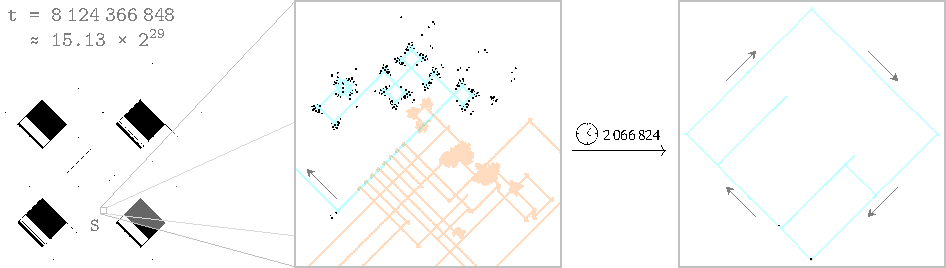
\includegraphics[width=1\textwidth]{0e0p/0e0p_timeline_8124366848.pdf}}
	\caption{The parent's control clock gun has destroyed most of its southern corner. The Herschel that is now present in it will send a glider counter-clockwise around its outer edge, destroying almost every other piece of the metacell over the next $2$ million generations.}
	\label{fig:0e0p_timeline_8124366848}
\end{figure}

Self-destruction continues through a few more stages past this point, with it being completely done at generation $t = 8{\thousep}129{\thousep}508{\thousep}130 \approx 15.1424 \times 2^{29}$, after which all parent metacells are gone, and only child metacells remain. The final clean-up step that occurs is a second glider escaping to the northwest from the south control clock, which destroys \texttt{INS}, where the single-channel glider recipe was injected into the nucleus (i.e., the area depicted back in Figure~\ref{fig:0e0p_timeline_974368517}).


%%%%%%%%%%%%%%%%%%%%%%
\subsection{Generations $\mathbf{16 \times 2^{29}}$ to $\mathbf{128 \times 2^{29}}$: Waiting and Repeating}\label{sec:0e0p_timeline_wait_repeat}
%%%%%%%%%%%%%%%%%%%%%%

If a child metacell's state is non-zero, it now spends an extraordinarily long time doing nothing of note---from generation $t = 16 \times 2^{29}$ until $t = 64 \times 2^{29}$ the gliders from the period $2^{29}$ control clock are blocked by a slow-salvo seed, so the contents of its nucleus simply cycle $48$ times without really doing anything.

On the other hand, if its state equals $0$, then the Herschel that is present in its south control clock at $t = 8{\thousep}589{\thousep}934{\thousep}592 = 16 \times 2^{29}$ releases a glider that uses one-time circuitry to (a) destroy the aforementioned slow-salvo seed, and (b) empty the contents of its nucleus. The result of (b) is that this metacell will not construct any children of its own, and the result of (a) is that it will self-destruct $47 \times 2^{29}$ generations sooner than it would otherwise (i.e., it acts as a ``dead'' cell). In the example that we are illustrating, none of the child metacells have state $0$, so this early death does not occur. However, we will see it occur in the next half-metageneration in Figure~\ref{fig:0e0p_timeline_34359738368}, $2^{35}$ generations from now.

\begin{figure}[!htb]
	\centering
	\embedlink{0e0p_timeline_34359738368_small}{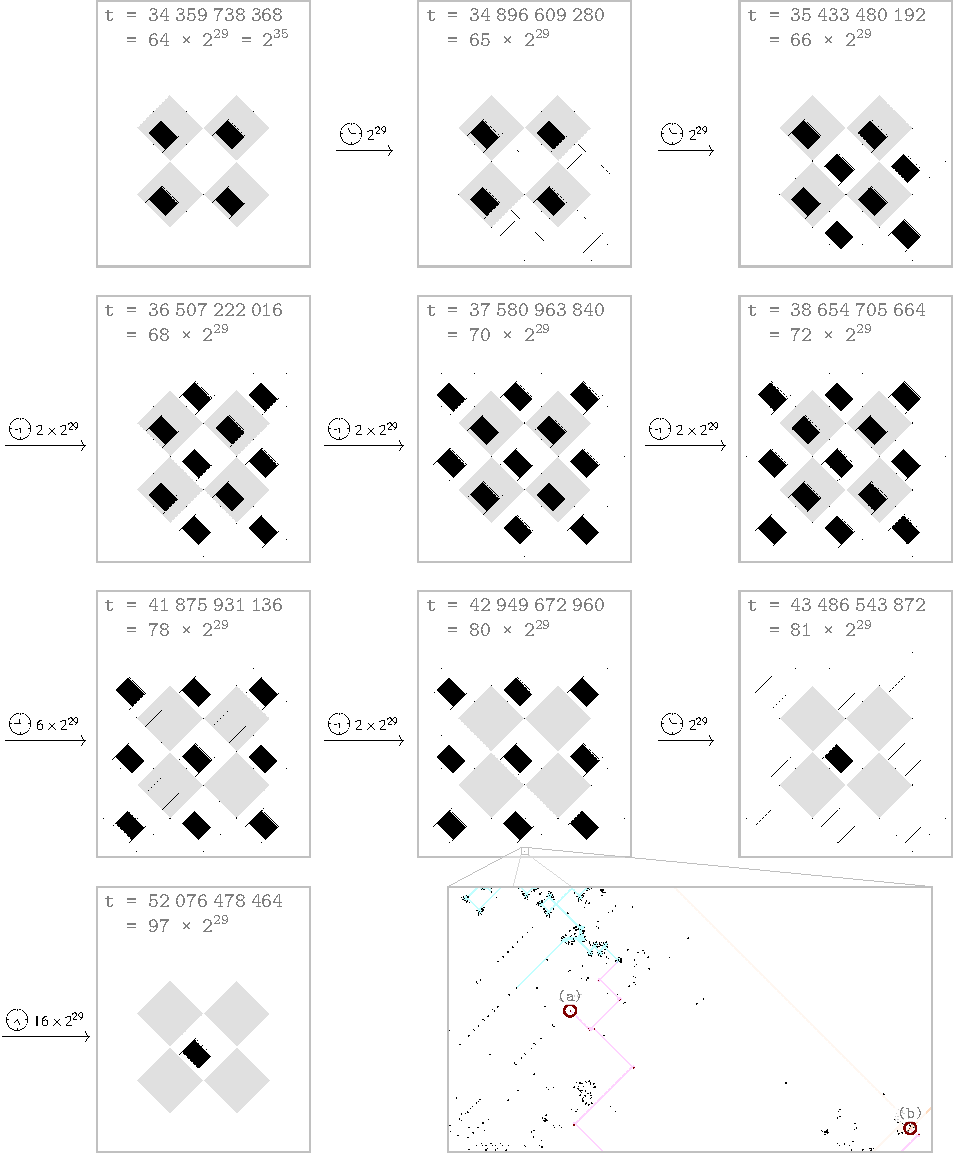
\includegraphics[width=1\textwidth]{0e0p/0e0p_timeline_34359738368.pdf}}
	\caption{The four children are now parents, so they construct their own children via the exact same stages that their parents used. In this example, $8$ of the $9$ grandchildren have state $0$, so they die early thanks to the Herschel that is present in the control clock gun at generation $80 \times 2^{29}$. That Herschel creates a glider that destroys (a) a block that would otherwise cause the grandchild to wait for $48 \times 2^{29}$ generations, and (b) a block in a syringe, so that the contents of the nucleus are absorbed by an eater~2.}
	\label{fig:0e0p_timeline_34359738368}
\end{figure}

At generation $t = 34{\thousep}359{\thousep}738{\thousep}368 = 64 \times 2^{29} = 2^{35}$, one half of a metageneration of the Moore-neighborhood cellular automaton (or equivalently, a full metageneration of the von-Neumann-neighborhood cellular automaton) has been completed, and child metacells are now in the same phase that the parent metacells were in at $t = 0$. All of the steps that we have seen so far now repeat, as these child metacells now start acting like parents (see Figure~\ref{fig:0e0p_timeline_34359738368}).

Only two aspects of this second half-metageneration differ from what we saw in the first half-metageneration:\footnote{Both of these differences \emph{can} happen in the first half-metageneration, but did not for us since we are only emulating a single cell.}\smallskip

\begin{itemize}
	\item \textbf{Multiple parents}: Some children are now located in positions that are adjacent to two or more parents. To prevent a parent from trying to construct a child that has already been constructed by another parent, the shell of each metacell simply has an eater in the path of incoming construction recipes, preventing them from doing anything.\smallskip
	
	\item \textbf{Early death}: Some children are constructed with state~$0$, so they die early.\smallskip
\end{itemize}

After all of this is complete, at $t = 68{\thousep}719{\thousep}476{\thousep}736 = 128 \times 2^{29} = 2^{36}$, a complete metageneration of the Moore-neighborhood rule is complete. In the particular rule that we are emulating here, a single live cell simply lives from one generation to the next, so we are left with a single copy of the 0E0P metacell that is identical to the one that we had at $t = 0$ (see Figure~\ref{fig:0e0p_timeline_68719476736}).

\begin{figure}[!htb]
	\centering
	\patternlink{0e0p_timeline_0_small}{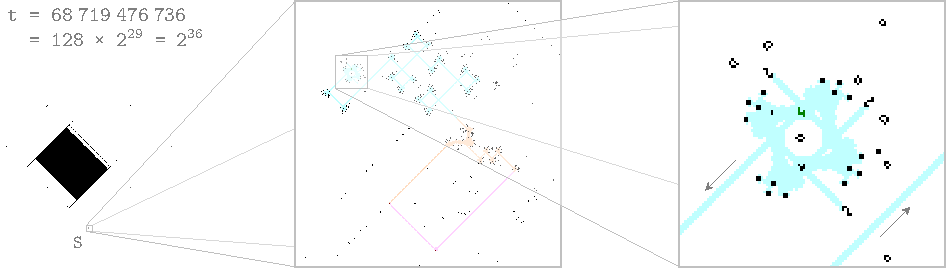
\includegraphics[width=1\textwidth]{0e0p/0e0p_timeline_68719476736.pdf}}
	\caption{A full metageneration of the $2$-state Moore-neighborhood rule has passed. In the particular rule being emulated here, a single cell lives from one generation to the next, so this snapshot is identical to the one from Figure~\ref{fig:0e0p_timeline_0}: a Herschel is present in the clock gun which will release a glider that will destroy an eater, eventually leading to the construction of its southeast neighbor.}
	\label{fig:0e0p_timeline_68719476736}
\end{figure}


%%%%%%%%%%%%%%%%%%%%%%%%%%%%%%%%
\section{Notes and Historical Remarks}\label{sec:0e0p_history}\index{metacell}
%%%%%%%%%%%%%%%%%%%%%%%%%%%%%%%%

Many metacells---patterns of size larger than $1 \times 1$ that emulate the behavior of a single cell---were constructed prior to 0E0P. The first one was the \textbf{p5760~metacell}, which was constructed by David Bell in January 1996. This metacell is much smaller and faster than 0E0P, with a period of just $5{\thousep}760$~generations and a bounding box size of just $500 \times 500$ (see Figure~\ref{fig:p5760_metacell}). However, there are numerous trade-offs that make this metacell less useful:\smallskip

\begin{figure}[!htb]
	\centering
	\begin{tikzpicture}
		\node[inner sep=0pt,anchor=south west] at (0,0) {\embedlink{p5760_metacell}{\patternimg{0.15}{p5760_metacell}}};
	
		\draw[white,line width=2.5pt,opacity=0.6](2.63,8.15) circle (0.2);
		\draw[redback2,line width=1pt](2.63,8.15) circle (0.2);
	\end{tikzpicture}
	\caption{The \emph{p$5760$~metacell}. Whether the cell is considered ``alive'' or ``dead'' is determined by the presence or absence of a glider at the location circled in \bgbox{redback}{red}. That glider, if present, is duplicated $8$ times and sent to its neighbors along the $8$ output paths highlighted in \bgbox{aquaback}{aqua}, signaling to them that it is alive. Similarly, neighboring alive cells send their signals to this one along the input paths highlighted in \bgbox{magentaback}{magenta}.}\label{fig:p5760_metacell}
\end{figure}

\begin{itemize}
	\item \textbf{Rule emulation}: It is hard-wired to emulate Life, and cannot easily be modified to emulate most of the other $2^{511}$ different zero-preserving 2-state Moore-neighborhood cellular automata.\smallskip
	
	\item \textbf{Visualization}: It is not easy to tell at a glance which ``cells'' are alive and which are dead---it is determined by the presence or absence of a single extra glider in the cell---and it is thus not interesting to look at from a far-out zoom level.\smallskip
	
	\item \textbf{Background grid}: ``Dead'' metacells must be placed on the Life plane, which means that, for example, spaceships cannot be emulated by this metacell unless the pattern is infinitely large.\smallskip
\end{itemize}

The first two of these problems were solved by the \emph{OTCA metapixel},\index{OTCA metapixel} which was constructed by Brice Due from late 2005 to mid-2006. While this metacell is a bit larger and slower than the first metacell (it is $2048 \times 2048$ and has period $35{\thousep}328$), it can be used to emulate any of the $2^{18}$ different outer-totalistic Life-like cellular automata. Indeed, built into its circuitry is an easily-adjustable array of eaters that determine how many live neighboring OTCA metapixels should lead to the birth or survival of the current metapixel (see Figure~\ref{fig:otca_metapixel}). 
% Introduce Life-like CA, since no introduction earlier
% mention out of the blue/honey bit/demultiplexer?

% FIGURE HERE, SHOWING PIXEL AND RULE ENCODINGS

The OTCA metapixel also has the remarkable feature that its alive and dead states look, from a distance, like alive and dead cells. This feature is achieved by the ``alive'' version of the cell releasing $43$ pairs of perpendicular lightweight spaceship streams that mutually annihilate each other, thus partially filling in the otherwise empty center of the metacell. For example, arranging a $1 \times 3$ row of ``alive'' metapixels (and a suitably large ``dead'' array of metapixels around its edges) results in a pattern that looks and evolves like a blinker, but $2{\thousep}048$ times as long and wide and $35{\thousep}328$ times as slow (see Figure~\ref{fig:metablinker}).

\begin{figure}[!htb]
	\centering
	\embedlink{metablinker}{\vcenteredhbox{\patternimg{0.104}{metablinker_0}} \vcenteredhbox{\color{black}{$\xrightarrow{\text{\clock{5}{46} 35328}}$}} \vcenteredhbox{\patternimg{0.104}{metablinker_35328}}}
	\caption{A \emph{metablinker}: an arrangement of OTCA metapixels that emulates a blinker, but with period $2 \times 35{\thousep}328$.}\label{fig:metablinker}\index{metablinker}
\end{figure}

The next notable metacell to be constructed was the \emph{p1 megacell},\index{p1 megacell} by Adam P.~Goucher in 2008. This metacell was, again, larger and slower than the metacells that came before it, with a bounding box of $2^{15} \times 2^{15}$ and a period of $2^{24}$. The new features this time that warranted the extra size and delay were twofold:\smallskip

\begin{itemize}
	\item This metacell was built entirely out of stable (p$1$) components like Herschel tracks, with the exception of a single period~$2^{24}$ gun used to regulate its timing.\footnote{This gun could be swapped out for a gun of another period, but periods that are multiples of $2$ help the pattern run quicker under the HashLife algorithm in Life simulation software like Golly.}\index{HashLife}\smallskip
	
	\item All $2^{512}$ non-outer-totalistic Life-like cellular automata can be emulated by this metacell, versus the $2^{18}$ outer-totalistic Life-like cellular automata that can be emulated by the OTCA metapixel.\smallskip% Maybe not-necessarily-outer-totalistic, instead of non-outer-totalistic?
\end{itemize}

% Figure of p1 megacell? Have had a lot of big figures bunched up closely here, so maybe not.

Finally, Adam P.~Goucher spent 2014--2018 constructing the 0E0P metapixel, which solved problem~(3) described earlier---it does not require a background grid of ``dead'' cells to be placed on the Life plane.

%https://www.conwaylife.com/forums/viewtopic.php?f=15&t=4117#p82954
%https://cp4space.hatsya.com/2018/11/12/fully-self-directed-replication/
%https://www.conwaylife.com/forums/viewtopic.php?f=2&t=3835
%https://www.conwaylife.com/forums/viewtopic.php?t=3968
%https://www.conwaylife.com/forums/viewtopic.php?p=72241

% EXERCISE: Give reactions in HighLife-replicator-ship.rle from Golly and ask reader to make ship out of it
% EXERCISE: Logarithmic replicator from B36/S245, found by Mark Niemiec in July 1994. Do... something with it. Pop in generation 300*4^n - 127 is 64 for all n >= 0.

% EXERCISE: There is *almost* an RRO in a Life-like, but just give a footnote/exercise about it. Exercise could ask why it's not a true RRO.
% EXERCISE: Show how iso in Moore neighborhood can emulate outer totalistic in von Neumann neighborhood
% EXERCISE: Give iso rulestring for (some rule)
% EXERCISE: Create a non-iso rule in which a single cell acts as... (diagonal spaceship, what else?)
% Exercise about emulating an elementary cellular automaton

% EXERCISE(S) about transition rules for rule emulation: find another one. Also:
% the different cell states, there are 200 different such functions sending 0 to 0.
% With 8 states we have 7 colors. Doing this with 6 or fewer colours is absolutely impossible, and with 7 colours is difficult (there are only 200 distinct solutions, or 13 up to rotation/reflection).
% EXERCISE: Describe positions of replicators in HashLife replicator? Connect to Sierpinski triangle maybe (same pattern as n-th row of it)
% Maybe exercise about 89-rotational RRO (https://www.conwaylife.com/forums/viewtopic.php?f=15&t=4116&p=131063#p131063). Or a part (b) of the already-planned RRO exercise?


%%%%%%%%%%%%%%%%%%%%%%%%%%%%%%%%%
\section*{Exercises \hfill \normalfont\textsf{\small solutions to starred exercises on \hyperlink{solutions_0e0p}{page \pageref{solutions_0e0p}}}}
\label{sec:solutions_0e0p}
\addcontentsline{toc}{section}{Exercises}
\vspace*{-0.4cm}\hrulefill\vspace*{-0.3cm}\footnotesize\begin{multicols}{2}\vspace*{-0.4cm}\raggedcolumns\interlinepenalty=10000
	\setlength{\parskip}{0pt}
	%%%%%%%%%%%%%%%%%%%%%%%%%%%%%%%%%
	
	
	\begin{problem}\label{exer:replicator_rule_really_replicates}
		Recall the replicator rule \texttt{B1357/S1357} that was illustrated in Figure~\ref{fig:replicator_smile}.\smallskip
		
		\begin{enumerate}[label=\bf\color{ocre}(\alph*)]
			\item \probdiff{2} If the longest side of a pattern's bounding box is $n$ cells long, how many generations would it take to copy itself for the first time in this rule?
			% Solution: 2^(ceil(log_2(n))) generations
			
			\item \probdiff{5} Prove that every pattern in this rule really does replicate, as we claimed.
			
			\noindent [Hint: First, prove (via induction, perhaps) that a single cell replicates. Then show that evolving a multi-cell pattern in this rule is equivalent to evolving each cell individually and XOR-ing the results together.].
		\end{enumerate}
	\end{problem}


	\mfilbreak
	
	
	\begin{problem}\label{exer:0e0p_single_cell_spaceships}
		Modify the rule used in Figure~\ref{fig:single_cell_knightship} so as to construct a (non-isotropic) 2-state cellular automaton on a square grid in which a single cell is a spaceship with speed...\smallskip
		
		\begin{enumerate}[label=\bf\color{ocre}(\alph*)]
			\item \probdiff{2} $c/2$ orthogonal;
			
			\item \probdiff{2} $c$ diagonal;
			
			\item \probdiff{2} $c/2$ diagonal; and
			
			\item \probdiff{4} $(1,3)c/4$ or any other non-orthogonal, non-diagonal, and non-knightship slope.
			
			\noindent [Hint: Use two generations to transform the cell into a domino, and two more generations to transform it back into a single cell.]
		\end{enumerate}
	\end{problem}
% SOLUTIONS: https://www.conwaylife.com/forums/viewtopic.php?f=11&t=3089&p=95700&hilit=MAP#p96359
% MORE: https://www.conwaylife.com/forums/viewtopic.php?f=11&t=3089&hilit=MAP&start=50#p98128


	\mfilbreak
	
	
	% TODO: Add solution
	\begin{problem}\label{exer:0e0p_rro_technicalities} \probdiff{3}
		Copies of the 0E0P metacell can be placed on the Life plane so as to evolve in the same way as the pattern from Figure~\ref{fig:reflectorless_rotating_oscillator1}.\smallskip
		
		\begin{enumerate}[label=\bf\color{ocre}(\alph*)]
			\item Explain why this pattern is \emph{not} a reflectorless rotating oscillator in Life, despite being a RRO in the rule that the 0E0P is emulating.
			% SOLUTION: metacell itself does not rotate
			
			\item Explain how you could use even more 0E0P metacells to emulate multiple copies of the pattern from Figure~\ref{fig:reflectorless_rotating_oscillator1} so as to create an actual RRO in Life.
			% Use four copies, rotated
		\end{enumerate}
	\end{problem}

	
	\mfilbreak
	
	
	\begin{problem}\label{exer:0e0p_single_cell_rro_rule}
		The 0E0P metacell from Figures~\ref{fig:0e0p_timeline_0}--\ref{fig:0e0p_timeline_68719476736} is emulating the isotropic rule
		\begin{align*}
			& \texttt{B2-an3-eiky4aiqw5ijnr6ak} \\
			& \quad \texttt{/S012ik3-acir4kqw5acq6ack7c8}.
		\end{align*}
		
		\begin{enumerate}[label=\bf\color{ocre}(\alph*)]
			\item \probdiff{2} Find an RRO in this rule.
			
			\item \probdiff{3} Use multiple copies of the 0E0P metacell (each emulating this rule) so as to create an RRO in Life.
			
			\noindent [Hint: Be careful and recall the solution of Exercise~\ref{exer:0e0p_rro_technicalities}.]
		\end{enumerate}
	\end{problem}


	\mfilbreak


	\begin{problem}\label{exer:0e0p_one_cell_smos}\index{spaceship made of spaceships} \probdiff{3}
		Create a von-Neumann-neighbourhood cellular automaton on a 2D square grid with at most $8$ states, where every cell dies in every generation (so it is of the type described in Section~\ref{sec:0e0p_rule_emulation} that can be emulated by the 0E0P metacell), in which two single-cell spaceships can collide so as to create a $2$-cell SMOS.
		
		\noindent [Hint: Make a cell in one state move south, a cell in another state move east, and something else happen when they collide.]
	\end{problem}
	% SOLUTION: https://www.conwaylife.com/forums/viewtopic.php?p=72241#p72170


	\mfilbreak
	
	
	\begin{problem}\label{exer:non_isotropic_rulestring_life} \probdiff{3}
		What is the non-isotropic rulestring (in the sense of Appendix~\ref{sec:non_isotropic_rulestrings}) for Conway's Game of Life?
	\end{problem}
	% SOLUTION: MAPARYXfhZofugWaH7oaIDogBZofuhogOiAaIDogIAAgAAWaH7oaIDogGiA6ICAAIAAaIDogIAAgACAAIAAAAAAAA
	
	
	\mfilbreak
	
	
	\begin{problemstar}\label{exer:0e0p_snark_destroyer} \probdiff{2}
		Recall that a single glider can destroy a Snark, as long as we place some extra still lifes near it as in Figure~\ref{fig:snark_seeded_destroy}.\smallskip
		
		\begin{enumerate}[label=\bf\color{ocre}(\alph*)]
			\item Find a similar configuration of still lifes that is used in the 0E0P metacell so as to allow a single glider to destroy a Snark.
			
			\item Explain why the configuration of still lifes from part~(a) might be preferable to the one from Figure~\ref{fig:snark_seeded_destroy}, despite being larger.
		\end{enumerate}
	\end{problemstar}


	\mfilbreak
	
	
	\begin{problem}\label{exer:0e0p_state_lookup_wider} \probdiff{2}
		The toy version of the state-lookup clock gun that we displayed in Figure~\ref{fig:state_lookup_clock_gun} extracts an approximately 100-generation chunk of a glider stream. Adjust its one-time circuitry so as to extract an approximately 900-generation chunk of a glider stream (which is large enough to store $0$--$7$ gliders, just like in the state-lookup mechanism of the 0E0P metacell itself).
	\end{problem}


	\mfilbreak
	
	
	\begin{problem}\label{exer:0e0p_why_blocks_clock_lane} \probdiff{2}
		In Figure~\ref{fig:0e0p_clock_gun_full}, we can see that stages $1$, $3$, $5$, and $7$ of a metacell's lifecycle (i.e., the stages where its newly-constructed children's nuclei are filled) are not initiated by the p$2^{29}$ clock gun---there are simply blocks in the output lane at those positions that absorb the output glider.
		
		\noindent Explain what \emph{other} mechanism is used to initiate those stages and redirect a copy of the single-channel glider recipe into the children's nuclei.
	\end{problem}
% SOLUTION: This is described in the text itself. Single leftover glider from long construction process is redirected back to parent to destroy a Snark at the edge of the parent's kernel.


	\mfilbreak
	
	
	\begin{problemstar}\label{exer:0e0p_extra_south_glider} \probdiff{2}
		In Figure~\ref{fig:0e0p_timeline_1040180152}, there is a one-time-turner that emits a glider to the south (first to the southeast, but it is then redirected to the southwest). What does this glider do, and what purpose does it serve?
	\end{problemstar}


	\mfilbreak
	
	
	\begin{problem}\label{exer:0e0p_how_make_faster} \probdiff{3}
		Describe at least three different ways that the 0E0P metacell could be modified so as to be smaller and/or faster, without sacrificing any of its functionality.
	\end{problem}
	% SOLUTION: Get rid of the various waiting stages, like stages 16-63. Optimize the single-channel construction recipe so as to use a better construction order. Update the single-channel construction recipe to use the c/4 wick-based elbow push instead of Cordership-based (may not be faster at distances used here, but certainly the 2-engine Cordership push would be an improvement over its 3-engine version). Likely a dozen other ways too. Another one: rewire so that nucleus is shut off at t = 8 * 2^29 instead of 13 * 2^29.
	
	
	%% EXERCISE END COMMANDS
\end{multicols}
\normalsize\vspace*{0.01cm}
%% DONE EXERCISE END COMMANDS
